% Opsætter KU Tex dokument
%%%%%%%%%%%%%%%%%%%%%%%%%%%%%%%%%%%%%%%%%%%%%%%%%%%%%%%%%%%%%%%%%%%%%%%%%%%%%%%%
\documentclass{article}                                                        %
\usepackage[a4paper, hmargin={2.8cm, 2.8cm}, vmargin={2.5cm, 2.5cm}]{geometry} %
\usepackage{eso-pic}  % \AddToShipoutPicture                                   %
\usepackage{graphicx} % \includegraphics                                       %
%\usepackage{subfig}    
\usepackage{setspace}                                                        %
%%%%%%%%%%%%%%%%%%%%%%%%%%%%%%%%%%%%%%%%%%%%%%%%%%%%%%%%%%%%%%%%%%%%%%%%%%%%%%%%

% Pakker til skrifttyper, tekst osv.
%%%%%%%%%%%%%%%%%%%%%%%%%%%%%%%%%%%%%%%%%%%%%%%%%%%%%%%%%%%%%%%%%%%%%%%%%%%%%%%%
    \usepackage[utf8]{inputenc}  % Implementere Unicode                        %
    \usepackage[T1]{fontenc}     % Unicode skrifttype fx. é skrives som 1 tegn %
    %\usepackage[danish]{babel}   % Dansk Ordbog                                %
    \usepackage{microtype}       % Forbedre linjeombrydningen                  %
    \usepackage{libertine}       % Skrifttype                                  %
%%%%%%%%%%%%%%%%%%%%%%%%%%%%%%%%%%%%%%%%%%%%%%%%%%%%%%%%%%%%%%%%%%%%%%%%%%%%%%%%

% Pakker til matematik og kode.
%%%%%%%%%%%%%%%%%%%%%%%%%%%%%%%%%%%%%%%%%%%%%%%%%%%%%%%%%%%%%%%%%%%%%%%%%%%%%%%%
    \usepackage{mathtools}       % Udvidelse til amsmath pakken                %
    \usepackage{amsthm}          % Pakke til bevisførelse                      %
    \usepackage{amssymb}         % Extra matematiske symboler                  %				
	\usepackage{mychemistry}												   %
	\usepackage[version=3]{mhchem}											   %
	\usepackage{wrapfig}													   %
	\usepackage{siunitx}	
	\usepackage{anyfontsize}
	\usepackage{url}
	\usepackage{ragged2e}
	\usepackage{algorithm2e}
	\usepackage[final]{pdfpages}
	\usepackage{listings}
	\usepackage{tikz}
	\usepackage{multirow}
	\usepackage{makecell}
	\usepackage{fourier} 
	\usepackage{array}
	\usepackage{todonotes}
	\usepackage{pdflscape}
	\usetikzlibrary{arrows,shapes}
	\usepackage{titlesec}
	\usepackage{hyperref}
	\usepackage{url}
	\usepackage[nottoc,numbib]{tocbibind}
	\usepackage{caption}
	\usepackage{subcaption}
	
	\usepackage{tikz}
	\usetikzlibrary{trees}
	\tikzset{level 1/.style={level distance=1.5cm, sibling distance=5cm}}
	\tikzset{level 2/.style={level distance=1.5cm, sibling distance=2cm}}
	\tikzset{bag/.style={text width=20em, text centered,yshift=-0.2cm}}
	
	\urlstyle{same}
	\tikzstyle{vertex}=[circle,fill=white!25,minimum size=20pt,inner sep=0pt]
	\tikzstyle{edge} = [draw,thick,-]

	\definecolor{light-gray}{gray}{0.85}
	\definecolor{dkgreen}{RGB}{0.0,128.0,43.0}
	\lstdefinelanguage{FSharp}%
{morekeywords={new, match, with, rec, open, module, namespace, type, of, member, % 
and, for, while, true, false, in, do, begin, fun, function, return, yield, try, %end
mutable, if, then, else, cloud, async, static, use, abstract, interface, inherit, finally, int },
  otherkeywords={ let!, return!, do!, yield!, use!, var, from, select, where, order, by },
  keywordstyle=\color{bluekeywords},
  sensitive=true,
  basicstyle=\ttfamily,
	breaklines=true,
  xleftmargin=\parindent,
  aboveskip=\bigskipamount,
	tabsize=4,
  morecomment=[l][\color{dkgreen}]{///},
  morecomment=[l][\color{dkgreen}]{//},
  morecomment=[l][\color{dkgreen}]{(*},
  morecomment=[s][\color{dkgreen}]{},
  morestring=[b]",
  showstringspaces=false,
  literate={`}{\`}1,
  stringstyle=\color{redstrings},
}
	
	\lstset{frame=tb,
  	language=[sharp]C,			%CHANGE LANGUAGE
  	aboveskip=3mm,
  	belowskip=3mm,
  	showstringspaces=false,
  	columns=flexible,
  	basicstyle={\small\ttfamily},
  	numbers=left,
  	numberstyle=\tiny\color{gray},
  	keywordstyle=\color{blue},
  	commentstyle=\color{dkgreen},
  	stringstyle=\color{red},
  	breaklines=true,
  	breakatwhitespace=true,
  	tabsize=3,
  	backgroundcolor=\color{light-gray},
	}
												   %
%%%%%%%%%%%%%%%%%%%%%%%%%%%%%%%%%%%%%%%%%%%%%%%%%%%%%%%%%%%%%%%%%%%%%%%%%%%%%%%%

% Pakker til layout.
%%%%%%%%%%%%%%%%%%%%%%%%%%%%%%%%%%%%%%%%%%%%%%%%%%%%%%%%%%%%%%%%%%%%%%%%%%%%%%%%
    \usepackage{fancyhdr}            % Gør det muligt at bruge sidehoveder     %
    \usepackage{graphicx}            % Mulighed for bl.a. \includegraphics     %
    \usepackage{colortbl}            % Hvis man vil farvelægge sine tabeller   %
    \usepackage{array}               % Gør miljøerne array og tabular bedre    %
    \usepackage{parskip}             % Første paragraf i afsnit indrykkes ikke %
    \usepackage{titlesec}            % Tilpassing af afstand mellem sektioner  %
    \usepackage[lastpage,user]{zref} % Side x af y                             %
%%%%%%%%%%%%%%%%%%%%%%%%%%%%%%%%%%%%%%%%%%%%%%%%%%%%%%%%%%%%%%%%%%%%%%%%%%%%%%%%


% Implementerer en række makroer og de pakker der er importeret
%%%%%%%%%%%%%%%%%%%%%%%%%%%%%%%%%%%%%%%%%%%%%%%%%%%%%%%%%%%%%%%%%%%%%%%%%%%%%%%%
    \pagestyle{fancy}                        % Implementerer sidehoved         %
    \lhead{University of Copenhagen}                % Venstre sidehoved               %
    \rhead{Casper Bresdahl, Karl Levinsen}                             % Højre sidehoved      %
    \cfoot{\thepage\ of \zpageref{LastPage}} % Side x af y                     %
    \newtheorem*{prp}{Propostion}            % Skaber nyt theorem  
    \renewcommand{\baselinestretch}{1.5}       %
%%%%%%%%%%%%%%%%%%%%%%%%%%%%%%%%%%%%%%%%%%%%%%%%%%%%%%%%%%%%%%%%%%%%%%%%%%%%%%%%

% Mindsker afstanden mellem sektioner
%%%%%%%%%%%%%%%%%%%%%%%%%%%%%%%%%%%%%%%%%%%%%%%%%%%%%%%%%%%%%%%%%%%%%%%%%%%%%%%%%%
\titlespacing\section{0pt}{12pt plus 4pt minus 2pt}{0pt plus 1pt minus 3pt}      %
\titlespacing\subsection{0pt}{12pt plus 4pt minus 2pt}{0pt plus 1pt minus 3pt}   %
\titlespacing\subsubsection{0pt}{12pt plus 4pt minus 2pt}{0pt plus 1pt minus 3pt}%
%%%%%%%%%%%%%%%%%%%%%%%%%%%%%%%%%%%%%%%%%%%%%%%%%%%%%%%%%%%%%%%%%%%%%%%%%%%%%%%%%%

%Ændrer størelsen på sections
%%%%%%%%%%%%%%%%%%%%%%%%%%%%%%%%%%%%%%%%%%%%%%%%%%%%%%%%%%%%%%%%%%%%%%%%%%%%%%%%%%
\titleformat{\section}
{\normalfont\fontsize{14}{16}\bfseries}{\thesection}{1em}{}
\titleformat{\subsection}
{\normalfont\fontsize{12}{14}\bfseries}{\thesubsection}{1em}{}
\titleformat{\subsubsection}
{\normalfont\fontsize{11}{13}\bfseries}{\thesubsubsection}{1em}{}
%%%%%%%%%%%%%%%%%%%%%%%%%%%%%%%%%%%%%%%%%%%%%%%%%%%%%%%%%%%%%%%%%%%%%%%%%%%%%%%%%%

%%%%%%%%%%%%
% Document %
%%%%%%%%%%%%

\begin{document}

\begin{titlepage}

\newcommand{\HRule}{\rule{\linewidth}{0.5mm}} % Defines a new command for the horizontal lines, change thickness here

\begin{center}
 % Center everything on the page
 
%----------------------------------------------------------------------------------------
%	HEADING SECTIONS
%----------------------------------------------------------------------------------------

\textsc{\LARGE University of Copenhagen}\\[1.5cm] % Name of your university/college
\textsc{\Large Computer Science}\\[0.5cm] % Major heading such as course name
\textsc{\large Bachelor Thesis}\\[0.5cm] % Minor heading such as course title

%----------------------------------------------------------------------------------------
%	TITLE SECTION
%----------------------------------------------------------------------------------------

\HRule \\[0.4cm]
{ \huge \bfseries Synthesis of Actor Code and tests =====TBD======}\\[0.4cm] % Title of your document
\HRule \\[1.5cm]
 
%----------------------------------------------------------------------------------------
%	AUTHOR SECTION
%----------------------------------------------------------------------------------------

\begin{minipage}{0.4\textwidth}
\begin{flushleft} \large
\emph{Authors:}\\ 
% Your name
Casper \textsc{Bresdahl} \\
Karl \textsc{Levinsen}
\end{flushleft}
\end{minipage}
~
\begin{minipage}{0.4\textwidth}
\begin{flushright} \large
\emph{Supervisor:} \\
Boris \textsc{Düdder}\\
\hfill
\end{flushright}
\end{minipage}\\[2cm]

% If you don't want a supervisor, uncomment the two lines below and remove the section above
%\Large \emph{Forfattere:}\\
%Axel \textsc{Christof}\\% Your name
%Casper \textsc{Bresdahl}\\
%Emilie \textsc{Bentsen}\\[1cm] 

%----------------------------------------------------------------------------------------
%	DATE SECTION
%----------------------------------------------------------------------------------------

{\large \today}\\[2cm] % Date, change the \today to a set date if you want to be precise

%----------------------------------------------------------------------------------------
%	LOGO SECTION
%----------------------------------------------------------------------------------------


\includegraphics{logo.png}\\[1cm] % Include a department/university logo - this will require the graphicx package
 
%----------------------------------------------------------------------------------------

\vfill % Fill the rest of the page with whitespace

%Disse linjer skaber forside, evt indholdsfortegnelse, og sætter sidetal
%%%%%%%%%%%%%%%%%%%%%%%%%%%%%%%%%%%%%%%%%%%%%%%%%%%%%%%%%%%%%%%%%%%%%%%%%%%%%%%%
									                                           %
    \thispagestyle{empty}   % Fjerner sidetal forside                          %
        % Slå disse til hvis der ønskes indholdsfortegnelse                    %
        %%%%%%%%%%%%%%%%%%%%%%%%%%%%%%%%%%%%%%%%%%%%%%%%%%%%%%%%%%%%%%%%%%%%%%%% 
            \newpage                % Side til indholdsfortegnelse            %
            \thispagestyle{empty}   % Fjerner sidetal fra indholdsfortegnelse %
            \tableofcontents        % Skaber indholdsfortegnelse              %
    \end{center}
    %\section*{Forord}
    	
		
        %%%%%%%%%%%%%%%%%%%%%%%%%%%%%%%%%%%%%%%%%%%%%%%%%%%%%%%%%%%%%%%%%%%%%%%%
    \newpage                % Første rigtige side
    \setcounter{page}{1}    % Sætter rigtigt sidetal på første side
%%%%%%%%%%%%%%%%%%%%%%%%%%%%%%%%%%%%%%%%%%%%%%%%%%%%%%%%%%%%%%%%%%%%%%%%%%%%%

\end{titlepage}
{\fontsize{10}{14}\selectfont

\section{Introduction} \label{intro}
In this thesis we have extended upon a sandbox like demo project from Microsoft \cite{AdventureGame} which resembles an adventure game and is written in a distributed fashion with Orleans. We have then decomposed it into a code repository with the  purpose of using the Combinatory Logic Synthesizer, a type based tool to automatically compose larger systems from a repository of code components, to create different variations of the game based on definitions written in a metalanguage. Our goal has been to synthesize code with timers, synthesizing code where we dispose timers, synthesizing code where we create other actors and to be able to define a list of parameters in our metalanguage and then synthesize code where only the defined parameters are present in the game variation. Our goal has also been to test our application, both as the initial program as well as the combinated variations of the game. This means synthesizing tests in the same way as our code, such that a given variation has tests alongside the program specific to that variation. 
\todo{Extend introduction to introduce testing?}\\
We will begin by looking at the theory behind the actor model and Orleans, then we will move to the theory of the Combinatory Logic Synthesizer and how it works. After that we will look into more detail about the extensions we have made to the Microsoft project. We will then look into the design decisions about decomposing the code, the issues we faced and what improvements we could have made. We will also look into what makes a good component and ask ourselves if we have achieved good decomposition. 
Then we will look into the relevant theory of testing software, followed by a deeper dive into our testing, meaning the tests themselves alongside the tests as combinators in the CLS. We will be discussing our implementation and looking at some of the obstacles we faced during our process of creating tests\todo{Change for a more comprehensive description}. We will then comment on our results and lastly make our conclusions.
\begin{itemize}
	\item Abstract
	\item Introduction
	\item Actor model - 4
	\item CLS - 4
	\item Our product - 4
	\item Discussion of implementation - 12
	\item Testing theory - 4
	\item Discussion of testing - 12
	\item Results - 4
	\item Conclusion
\end{itemize}
\section{Actor model}
The actor model is a programming model utilising concurrent computation for developing parallel, distributed and mobile systems. An actor can do three things: it can send messages to other actors, it can update its local state or it can create more actors. All actors work concurrently and asynchronously together by sending and receiving messages. When an actor receives a message it performs some specified task based on its local state and the content of the received message. This task can be to perform some computation, and the result can then be passed along to another actor in a new message \cite{ActorModelPaper}.\\
All actors have a globally unique name which is used to determine to which actor a message is sent. Name of actors may be communicated in messages such that an actor knows who to send the next message to, or such that an actor knows who just sent it a message. An actor's state is local and can not be shared with other actors, and thus, to change the behaviour of an actor, another actor must send a message specifying it to change state. The path a message takes and what network delays a message may encounter is not specified and thus messages may arrive out of order \cite{ActorModelPaper}.\\
\begin{figure}[H]
	\centering
	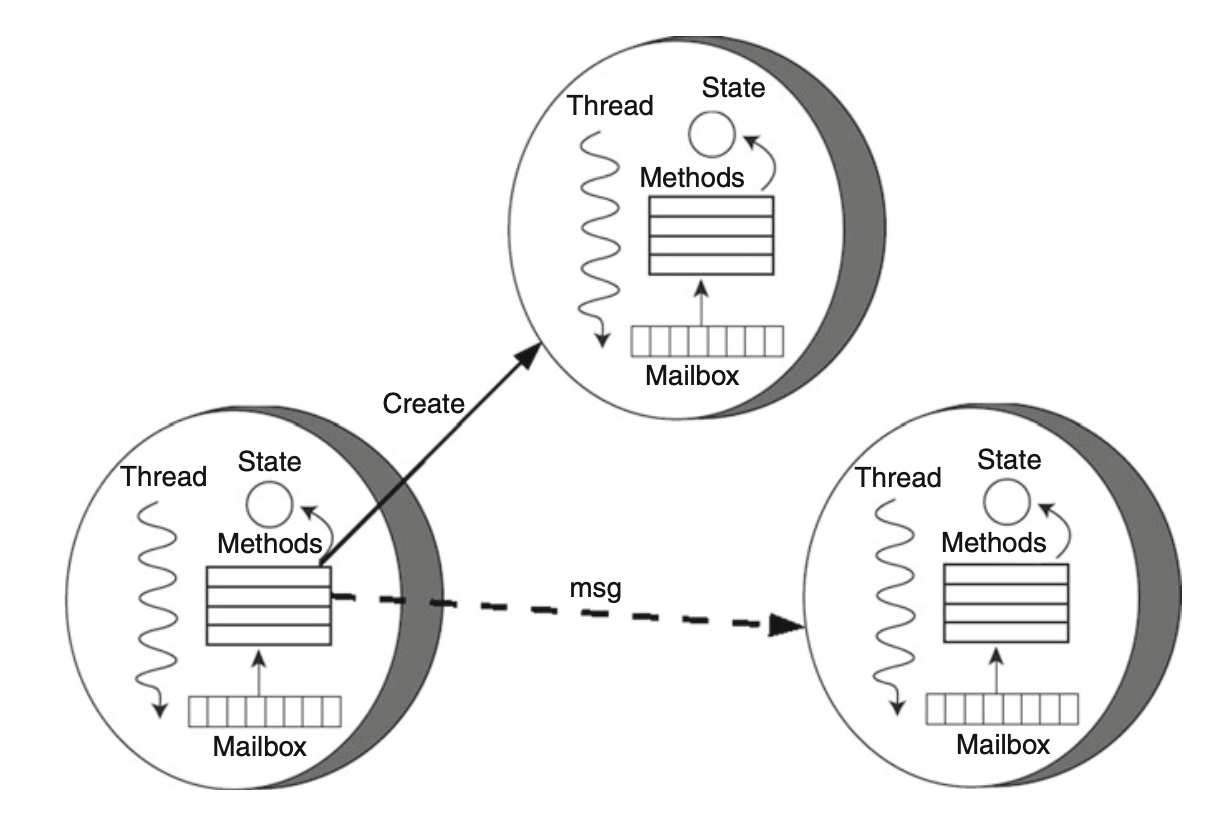
\includegraphics[width=0.85\linewidth]{Materials/ActorModel/AMDemonstrated}
	\caption{An actor consists of methods, a mailbox for queued messages and a local state. Actors can send messages, change state based on a received message and create other actors. Figures is from \cite{ActorModelPaper}.}
	\label{AMDemonstrated}
\end{figure}
As seen in \autoref{AMDemonstrated} an actor can be illustrated as an entity with a mailbox, a set of methods and a local state. The mailbox is often implemented as a queue \cite{ActorModelPaper}, and is used to store messages which arrive while the actor is already handling another message. The methods may make the actor change its state, make the actor create a new actor or send a message to another actor.\\
As already hinted at above, the core semantic properties of an actor are \textit{encapsulation} of the local state, the ability to \textit{atomically} execute methods, \textit{fairness} in scheduling actors and \textit{location transparency} to enable distributed execution and mobility \cite{ActorModelPaper}, and all of these we will look into next.
 
\subsubsection{Encapsulation and Atomicity}
Encapsulation means each actor has its own state, and thus all changes to the state of an actor has to come in a message sent from another actor. The notion of encapsulation is also one of the corner stones of object oriented programming where each object also has its own state. This can be very useful to enforce an object oriented decomposition in code, and may make actors look a lot like objects \cite{ActorModelPaper}.\\
Encapsulation has also lead to the notion of atomicity. In a sequential program one object may call a method in another object. This method will then run to the end before another object can call the method again. The called object may or may not have changed state during the method call, but we can only reason about this because the method call can not be interrupted by another method call. Because all method calls are run uninterrupted, we can reason about the object's behaviour given we know its state prior to the method call \cite{ActorModelPaper}.\\
In a concurrent setting an object may call a method in another object, but right after a third object does the same. If the first method call would be interrupted to accommodate the second, the object's state might already be altered, and we can no longer reason about the behaviour the object exhibits after a call to its method. This would lead to inconsistencies in the system as these concurrent calls can happen at any time. To guarantee we can reason about object behaviour in actors we therefore must guarantee that received messaged are handled atomically, meaning that the processing of a message happens in one step, and is not interrupted by new messages. This ensures that the encapsulated state is consistent throughout the execution of a program \cite{ActorModelPaper}.

\subsubsection{Fairness}
The notion of fairness states that all actors are scheduled time to run, and that they will make progress given they have computations to do. It also states that all messages are guaranteed to reach their destination unless that actor has been permanently disabled. The notion of fairness allows us to reason about the liveness properties of actor programs \cite{ActorModelPaper}. Here we note that an actor program is started by an external message sent to an actor, and that an actor program terminates when all actors are idle and no external message can be passed to any actors. An actor is considered idle if it has no pending messages in its mailbox.

\subsubsection{Location transparency}
Location transparency provides an abstraction for the programmers who need to make actors communicate. In the actor model the location of actors does not determine its name. Two actors might run on the same computer in the same core, or they might run on two different machines in two different countries. Location transparent naming enables the programmers no to worry about the actors physical location. \cite{ActorModelPaper}.\\
Mobility is defined as the ability for a computation to migrate to another node \cite{ActorModelPaper}. This is important for load-balancing, fault-tolerance, and reconfiguration, and is useful in achieving scalable performance \cite{ActorModelPaper} as an actor lifting a lot of heavy work along other actors doing the same on the same machine can seamlessly be moved to another machine in an attempt to alleviate the workload on that machine.

\subsubsection{Synchronization}
\begin{figure}[H]
	\centering
	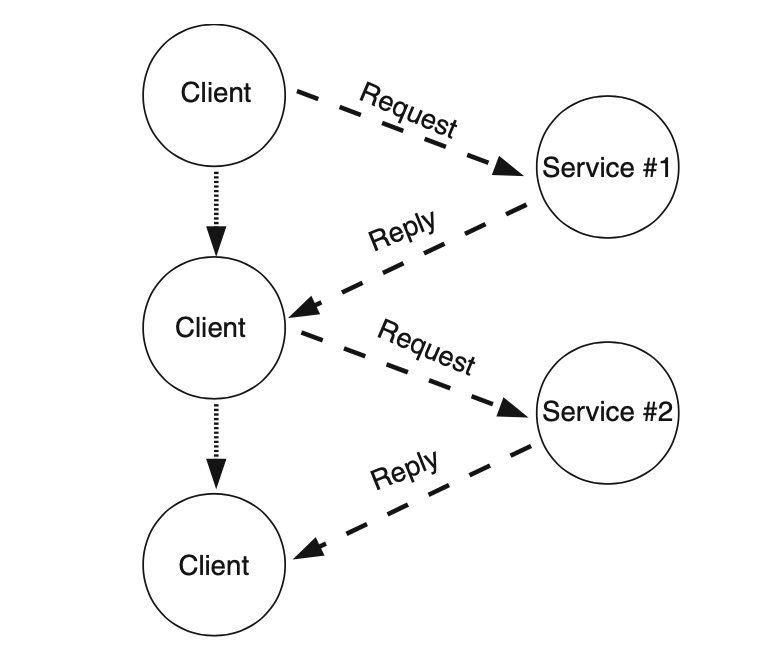
\includegraphics[width=0.6\linewidth]{Materials/ActorModel/AMCommunication}
	\caption{An illustration of how RPC like communication works. Figures is from \cite{ActorModelPaper}.}
	\label{AMCommunication}
\end{figure}
One way to achieve synchronization of actors is through Remote Procedure Call like message passing (RPC), which is a common communication pattern in actor systems \cite{ActorModelPaper}. In a situation where an actor wants to make sure another actor has received its message before it communicates it to others or where the order of messages matter RPC like messaging is a big help. In RPC like communication the sender of a message waits for a reply before it continues to process other messages. An actor might want to wait for a reply if it needs the information in the reply to continue its computation. This can be seen in \autoref{AMCommunication} where the client sends a message to a service and waits for the reply before sending another message to another service \cite{ActorModelPaper}.\\

\subsection{Orleans}
Orleans is a framework for C\# developed by Microsoft. The framework simplifies several aspects of the actor model to make it a lot easier for programmers to write actor based code. Some of the simplifications Orleans helps with are lifecycle management of actors in the application code, to deal with distributed race conditions, to handle failures and recovery of actors after server crashes, and to make an abstraction for actor placement.\\
An important abstraction the developers of Orleans have made is the notion of virtual actors. In Orleans we work with virtual actors which are based on the actors described previously, but they implement some important differences which abstract away some of the more cumbersome implementations of actors. The first of these is perpetual existence which states that virtual actors are logical entities which always exists. A virtual actor can not explicitly be created or destroyed. Its existence is unaffected by the server which runs it, and thus also unaffected by the server crashing. Given that a virtual actor always exists, it is also always addressable \cite{OrleansPaper}.\\
Another great help Orleans implement is automatic instantiation. The Orleans' runtime automatically creates instantiations of actors called activations. An actor can only be instantiated if it has a request pending. When a request is sent to an actor the Orleans runtime automatically instantiates an activation on a server. If the server should later crash, the Orleans runtime automatically re-instantiates the actor when the next request to it arrives. This means that the programmer does not have to program actor lifecycles themselves, but can rely on Orleans to automatically figuring out where and when to instantiate an actor. Likewise, the Orleans runtime also automatically disposes unused actors if they have been idle for a long time \cite{OrleansPaper}.\\
Orleans also takes care of the location transparency abstraction. An application running inside an actor, or communicating with an actor does not know its physical location, and neither does it need to, as long as it knows the actors name it can send it a message. Orleans allow programmers to name actors much like one would name an object in an ordinary object-oriented program.\\
Orleans allows for timers which, as the name suggests, specify code that will be run later. A timer is automatically disposed if an actor is recycled by runtime, but can otherwise be specified to fire in even intervals. Because timers 'run in the background' it is important that the programmer makes sure they are disposed when no longer needed.\\
Orleans allows actors to synchronize through RPC-like message passing as discussed in subsection '\nameref{Synchronization}'. This is done by awaiting a response from another actor. Due to atomicity the actor can not progress its method while awaiting a response. Therefore other actors or other tasks are run in the mean time while the actor waits. When the response arrives the actor will then continue the method from where it left off.
\section{Combinatory Logic Synthesizer}
A central part of our work involves the Combinatory Logic Synthesizer (CLS) which is a type based tool to automatically compose larger systems from a given repository consisting of components suited for synthesis. CLS has its roots from combinatory logic synthesis which is a type theoretic approach where a repository of components is used to achieve a synthesis \cite{CLSPaper}. Components are in this approach represented by components which consists of a name and an intersection type. The intersection type both catches the components actual type, but also its semantic type, describing its intended usage \cite{CLSPaper}. We can now look to the relativized inhabitation problem which asks the question: given a repository $\Gamma$ consisting of typed components, and a type we wish to reach, $\tau$, does there exist an inhabitant \textit{e} with type $\tau$ under the type assumptions of $\Gamma$? \cite{CLSPaper} In our work to synthesize a distributed system this is the exact question we would like answered, and it is the question the CLS answers. It is therefore important we understand how the CLS works.

\subsection{Composition synthesis}
In a type oriented approach types are constructed from constants (a), variables ($\alpha$) or function types ($\tau \to \tau'$) \todo{Wrong arrow. Does it matter?}. Terms can be constructed by using application for instance \textit{e} to \textit{e'}, or by using named components or combinators \cite{CLSPaper}. This can also be viewed as:
\begin{align*}
	&\text{Types}\; \tau,\;\tau'\; ::=\; a | \alpha | \tau \to \tau'\\
	&\text{Terms}\; e,\; e'\; ::= (e\; e') | X
\end{align*}
Composition synthesis consists of a single rule in its minimal form. This rule can be viewed logically under the Curry-Howard isomorphism as modus ponens \cite{CLSPaper}:
\begin{equation*}
	\frac{\Gamma \vdash F\; : \; \tau' \to \tau \quad \Gamma \vdash G\; : \; \tau'}{\Gamma \vdash (F\; G)\; : \; \tau}
\end{equation*}\todo{Do we need the var rule?}
Here we have two premises, that we have a variable \textit{G} in our repository $\Gamma$ of type $\tau'$ and that we have a function type \textit{F} in the same repository which takes a variable of type $\tau'$ to a variable of type $\tau$. If our premises hold, we can then by applying \textit{F} on \textit{G} create a variable in $\Gamma$ of type $\tau$.\\
We can now formulate the relativized inhabitation problem in a more mathematical sense, as it can be described as:
\begin{equation*}
	\exists e.\ \Gamma \vdash e\; : \; \tau?
\end{equation*}
Which reads: does there exists a composition \textit{e} in $\Gamma$ such that $\Gamma \vdash e\; : \; \tau$? An inhabitation algorithm is then used to synthesize an \textit{e} from $\Gamma$ and $\tau$. This makes the foundation of automatic synthesis \cite{CLSPaper}.

\subsection{Example of combinatory logic synthesis}
As an example of combinatory logic synthesis we can look at how our repository for the player object looks at time of writing (May 7, 2020). Our repository consists of nine functions based in four categories. At the top level we have a PlayerGrain which takes three strings into a MyResult object which is the native class we are looking for in our synthesis. We then have three ability functions, which each produces the string needed to synthesize that ability. The next three functions are then the case implementations needed to call the functions when the game is running. Lastly we have two functions which produces two different ways for the player to take damage. The repository can be seen in \autoref{playerRepo}.
\begin{figure}[H]
	\centering
	\begin{alignat*}{2}
	&\text{PlayerGrain}\; &&\text{: string, string, string} \to \text{MyResult}\\
	&\text{abilityFireball}\; &&\text{: void} \to \text{string}\\
	&\text{abilityRoar}\; &&\text{: void} \to \text{string}\\
	&\text{abilityNone}\; &&\text{: void} \to \text{string}\\
	&\text{caseFireball}\; &&\text{: void} \to \text{string}\\
	&\text{caseRoar}\; &&\text{: void} \to \text{string}\\
	&\text{caseNone}\; &&\text{: void} \to \text{string}\\
	&\text{damageTakenRoar}\; &&\text{: void} \to \text{string}\\
	&\text{damageTakenStandard}\; &&\text{: void} \to \text{string}
	\end{alignat*}
	\caption{The functions which make up the player repository at time of writing.}
	\label{playerRepo}
\end{figure}

Although \autoref{playerRepo} gives an overview of what has been implemented and it is possible to some extend to guess how these functions are grouped, semantic information seems to be missing. Just looking at our repository does not show very clearly, if at all, how the ability, case and damageTaken functions make three groups which makes a player. To show the semantics of our repository we make a taxonomy of it as seen in \autoref{taxonomy}. We here define dashed lines as a 'has a' relation and solid lines as a 'is a' relation. This means that player has a case, ability and a damageTaken component which each can take different forms. What we can not see in this representation is the 'horizontal' correlation between components. If the player has a fireball ability, the player needs to implement the fireball case and the standard damageTaken. Although this can not be seen, in the implementation these correlations has been made with kindings.

\begin{figure}[H]
	\centering
	\begin{tikzpicture}[grow=down, -stealth]
	\hspace{-2cm}
	\node[bag]{Player} 
	child[dashed]{;\node[bag]{Case}
		child[solid]{; \node[bag]{None}}
		child[solid]{; \node[bag]{Fireball}}
		child[solid]{; \node[bag]{Roar}}
	}
	child[dashed]{;\node[bag]{Ability}
		child[solid]{; \node[bag]{None}}
		child[solid]{; \node[bag]{Fireball}}
		child[solid]{; \node[bag]{Roar}}
	}
	child[dashed]{;\node[bag]{DamageTaken}
		child[solid]{; \node[bag]{Standard}}
		child[solid]{; \node[bag]{Roar}}
	};
	\end{tikzpicture}
	\caption{Taxonomy describing semantics about the player repository at time of writing.}
	\label{taxonomy}
\end{figure}

A central idea to the CLS is to combine semantic information together with the actual types when creating a repository \cite{CLSPaper}. We can do this by intersecting the repository in \autoref{playerRepo} with the taxonomy from \autoref{taxonomy}. This will add the missing semantic information we were looking for when we looked at the repository by itself. By intersecting native classes with semantic information we get the new repository in \autoref{intersectionRepo}.
\begin{figure}[H]
	\centering
	\begin{alignat*}{2}
	&\text{PlayerGrain}\; &&\text{: string $\cap$ case, string $\cap$ ability, string $\cap$ damageTaken} \to \text{MyResult $\cap$ player}\\
	&\text{abilityFireball}\; &&\text{: void} \to \text{string $\cap$ ability}\\
	&\text{abilityRoar}\; &&\text{: void} \to \text{string $\cap$ ability}\\
	&\text{abilityNone}\; &&\text{: void} \to \text{string $\cap$ ability}\\
	&\text{caseFireball}\; &&\text{: void} \to \text{string $\cap$ case}\\
	&\text{caseRoar}\; &&\text{: void} \to \text{string $\cap$ case}\\
	&\text{caseNone}\; &&\text{: void} \to \text{string $\cap$ case}\\
	&\text{damageTakenRoar}\; &&\text{: void} \to \text{string $\cap$ damageTaken}\\
	&\text{damageTakenStandard}\; &&\text{: void} \to \text{string $\cap$ damageTaken}
	\end{alignat*}
	\caption{The functions together with semantic information which make up the player repository at time of writing.}
	\label{intersectionRepo}
\end{figure}

With this new repository we can now find a meaningful composition which returns a player with a fireball ability by constructing the inhabitant \textit{PlayerGrain(caseFireball(), abilityFireball(), damageTakenStandard())} of type MyResult $\cap$ player. More formally we can call the repository from \autoref{intersectionRepo} $\Gamma$, and the composition thus becomes:
\begin{equation*}
	\Gamma \vdash \textit{PlayerGrain(caseFireball(), abilityFireball(), damageTakenStandard())}\; :\; \textit{MyResult}\cap \textit{player}
\end{equation*}

\section{The adventure game}
In our work with the CLS we have been working on creating an adventure game where the CLS would allow us to create different variations of the game based on the repository of code we have build. We have not build the game from the ground up, but instead we have taken a demo project from the Orleans documentation \cite{AdventureGame} and extended it. This was done to save development time and thus to reach a point where we could begin creating combinators faster and have a more 'real world like' system to work with. The original system involved players, monsters and rooms where all players and monsters would have one health. Things or items were scattered across the rooms and the player could pick them up. Most noticeably is the knife which allows a player to stab other players or monsters. The player and monsters could then move around the rooms, but the monsters would never attack \todo{Is this true?}. The game had no objective and no way to win. It served as a 'sandbox' project. There were more smaller implementations which were part of the original game, but because these have little to no relevance to our project we will leave them out of this overview.\\
The first extension to the game was the addition of health for both the player and monsters. This allowed us to interact in a more fine grained manner with the monsters, and opened up the possibilities of adding abilities to the player. We also extended the monster such that it would attack the player. These two additions makes our foundation for the game, and is what we would like to call our \textit{initial application} as everything else we have created revolves around this foundation.\\

With our extensions the game still has no objective. Our extensions have served only to show the use of the CLS tool to create and test actor code. The game is thus still a sandbox and can not be won.\\
We have extended the player with two abilities. The first is a fireball which deals high damage. The other ability is a roar which makes the player take half damage and healing for ten seconds. Both abilities have a cooldown (time before the ability can be used again). The idea is the player has either the fireball ability, the roar ability or neither, and that we achieve this through CLS.\\
The boss is an extension entirely created by us. The boss is a strong enemy which can spawn small monsters and has a lot of health. Further we have created two abilities for it, one which heals all other monsters in the room, and one where the boss takes half damage if there are monsters in the room with it. Again the idea is that through the use of CLS the boss either has one of the two abilities or is not in the game at all.\\
The room has been extended with weather effects. We have created four different weather effects which effects the player differently every time it enters a room. We have \textit{blizzard} which deals five damage to the player. \textit{Sunny} which heals the player for ten health. \textit{Cloudy} which does nothing and \textit{night} which makes it so the player gets fewer details about the room when it enters. The idea is that a random weather from a pool of available weathers (we get to this in \autoref{Metalanguage}) is chosen each time the player enters a room.\\

\begin{figure}[H]
	\centering
	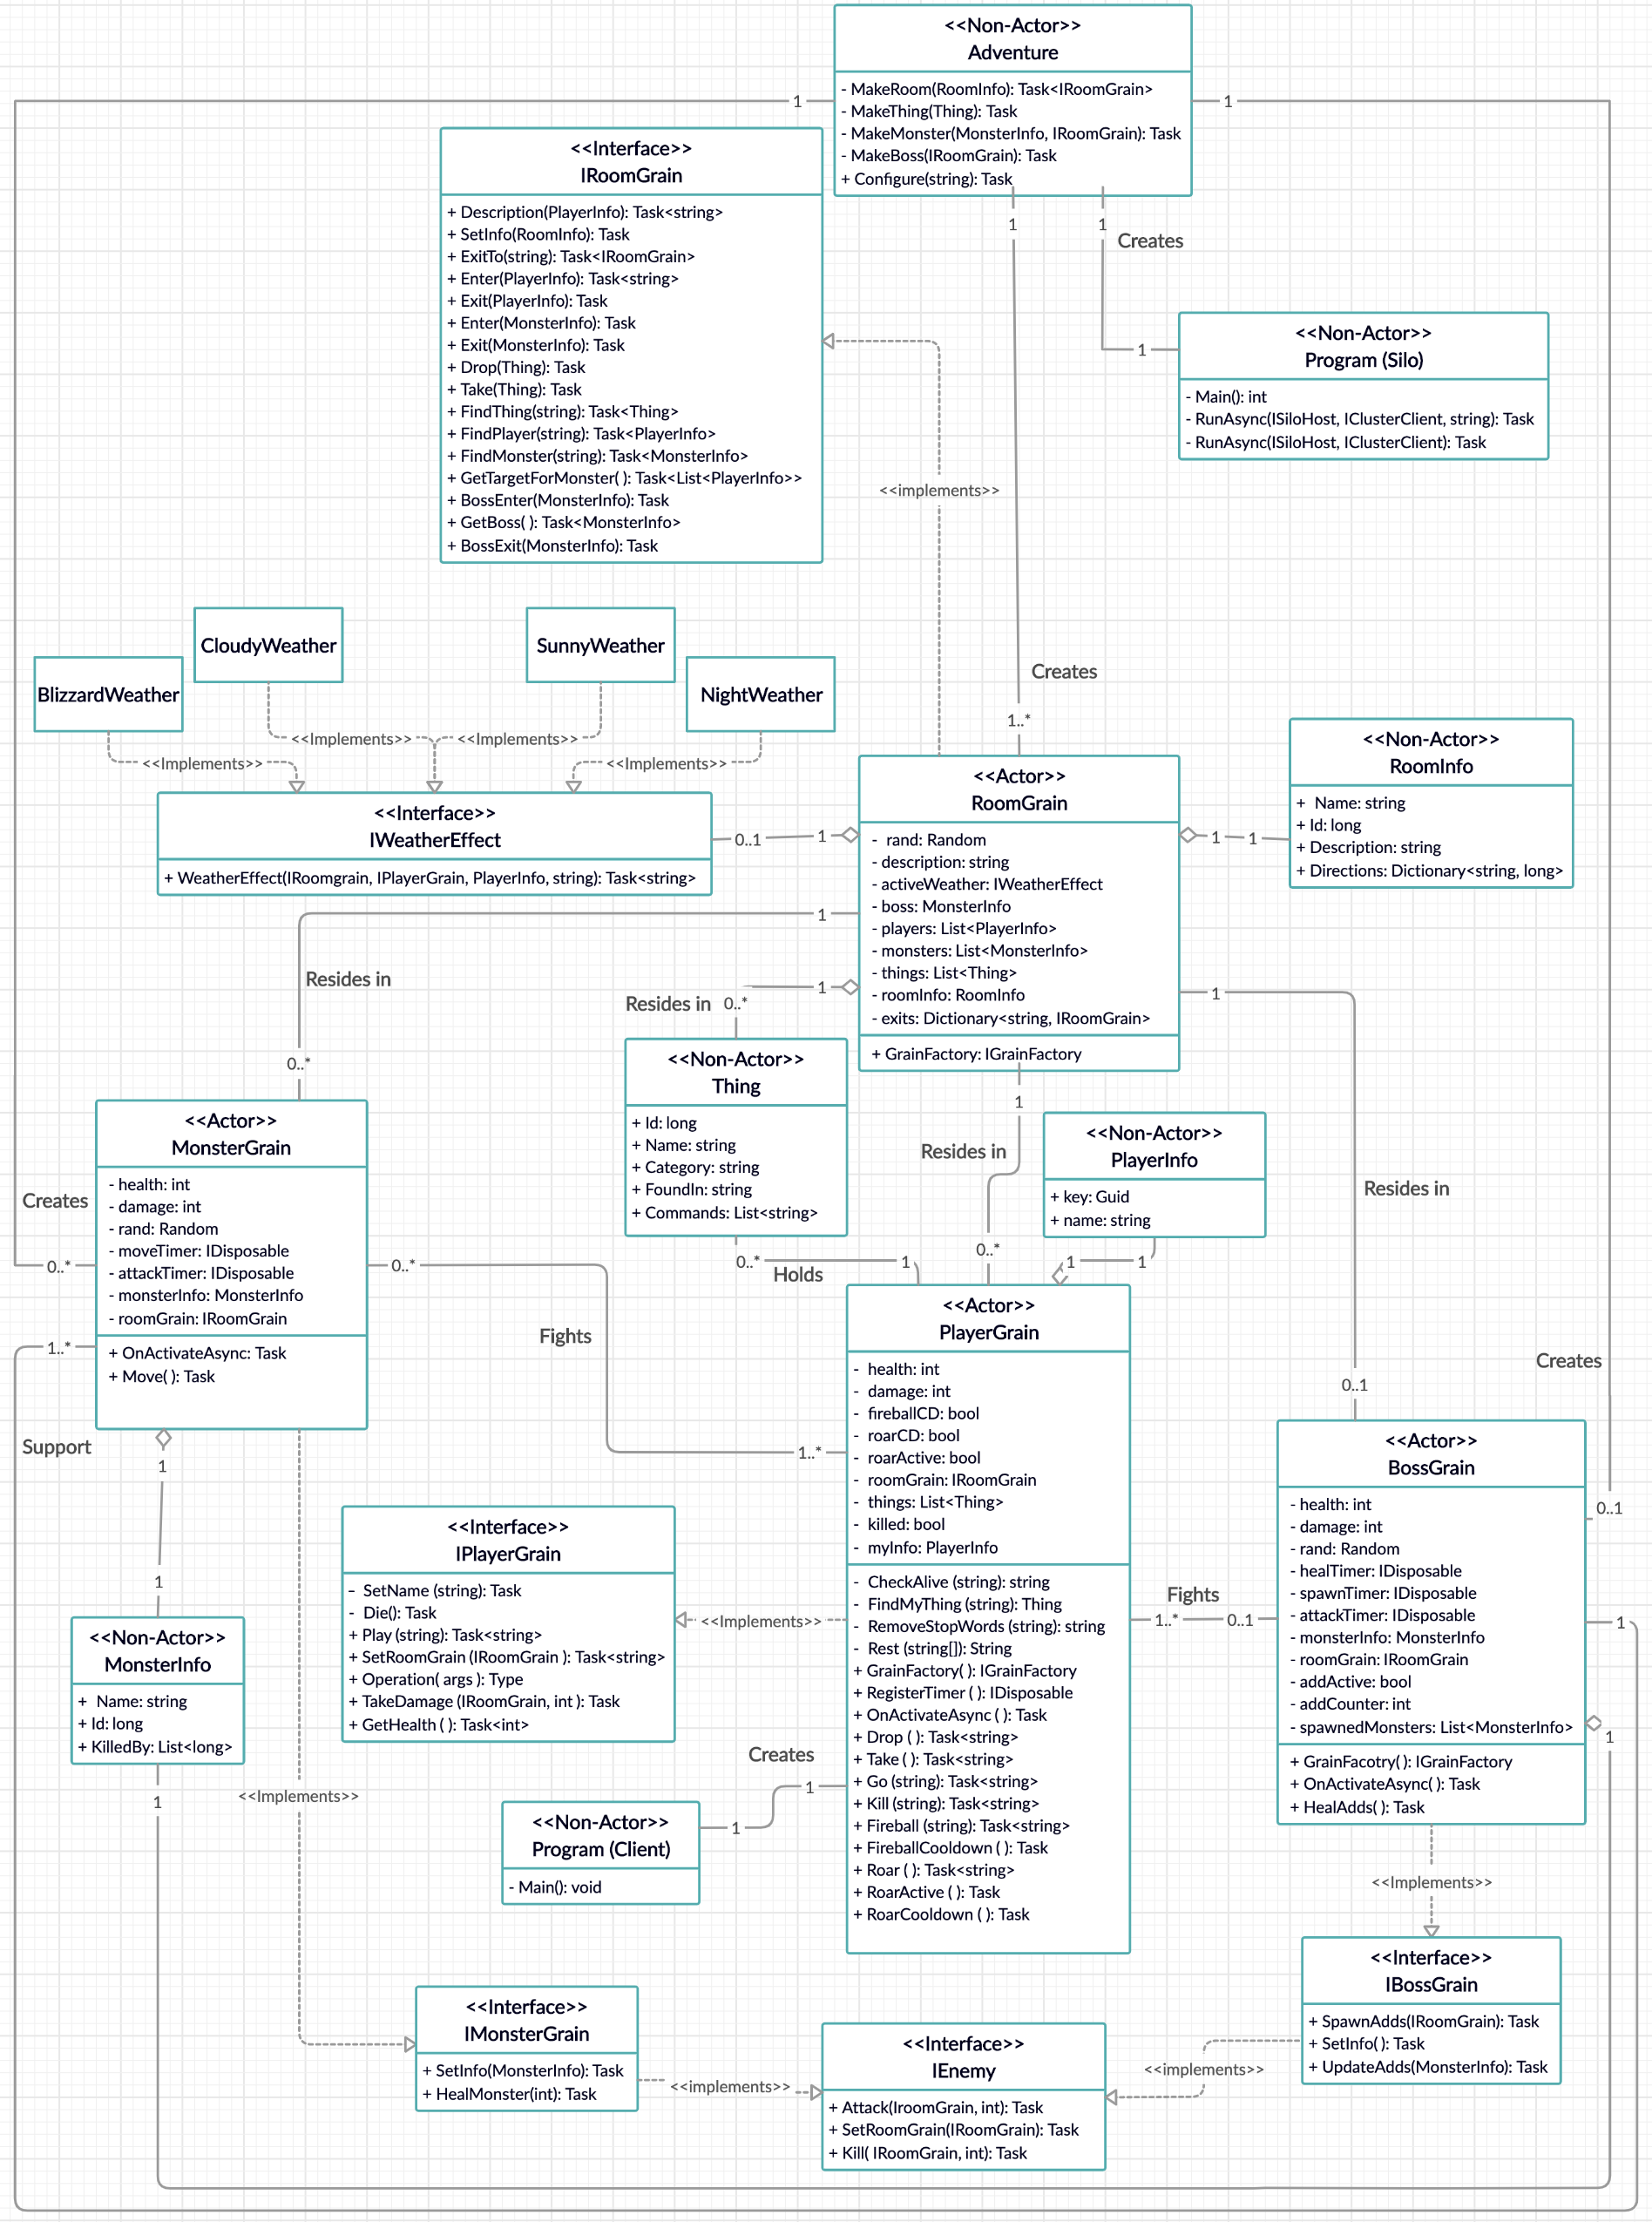
\includegraphics[width=\linewidth]{Materials/Adventuregame/ClassDiagram}
	\caption{UML class diagram of the adventure game with all extensions available.}
	\label{UML}
\end{figure}
In \autoref{UML} we see an UML class diagram for the whole game with all extensions. We see that there is quite high coupling between the room and the other actors, and in general a lot of communication the actors between. The room object works as a mediator object, and holds information about everyone in the room. The other objects do not know of each other, but instead asks the room if a player or specific monster is in the room with them. Because of this the room will receive a lot of communication as for all tasks involving more than one actor, the room will be prompted. However, as the there are a lot of rooms, we can not talk about a bottleneck. If we were to scale the game with a lot of players and monsters, we would likely scale the number of rooms proportionally, and so there will not be a lot of communication to one specific instantiation. In addition, the communication with the room is in general short, for instance when a player wants to fireball a monster. In \autoref{PLayerFireballFlow} we see a sequence diagram of a player using fireball on a monster. The player first asks the room to find players of the target's name, as there are none, the player then asks for monsters of the same name. This time there is one and the player can then tell the monster to take damage. As we see these lookups are only calls to a single function, and thus the communication is short.\\
If we look at the communication between the boss and the monsters it is only one way. The boss holds its own list of monsters it has spawned and thus does not need to prompt the room for what monsters are present. The room does however communicate to the boss when a monster dies in the room such that it can update its list. The boss can now go through its list of monsters and on for each tell it to heal. The boss does only have communication with monsters it spawns, not with the monsters found around the world.\\

\begin{figure}[H]
	\centering
	\includegraphics[width=\linewidth]{example-image-a}
	\caption{A sequence diagram showing the communication needed for the player to fireball a monster.}
	\label{PLayerFireballFlow}
\end{figure}

\subsection{Metaprogramming} \label{Metalanguage}
We have already talked about what variations are possible to create, but we have not gone into detail about how to achieve them. To create the variation of our adventure game we want, we need a \textit{'reference client'}, a template for what the CLS should be looking for.
\begin{wrapfigure}{L}{0.6\linewidth}
	\vspace{-10px}
	\centering
	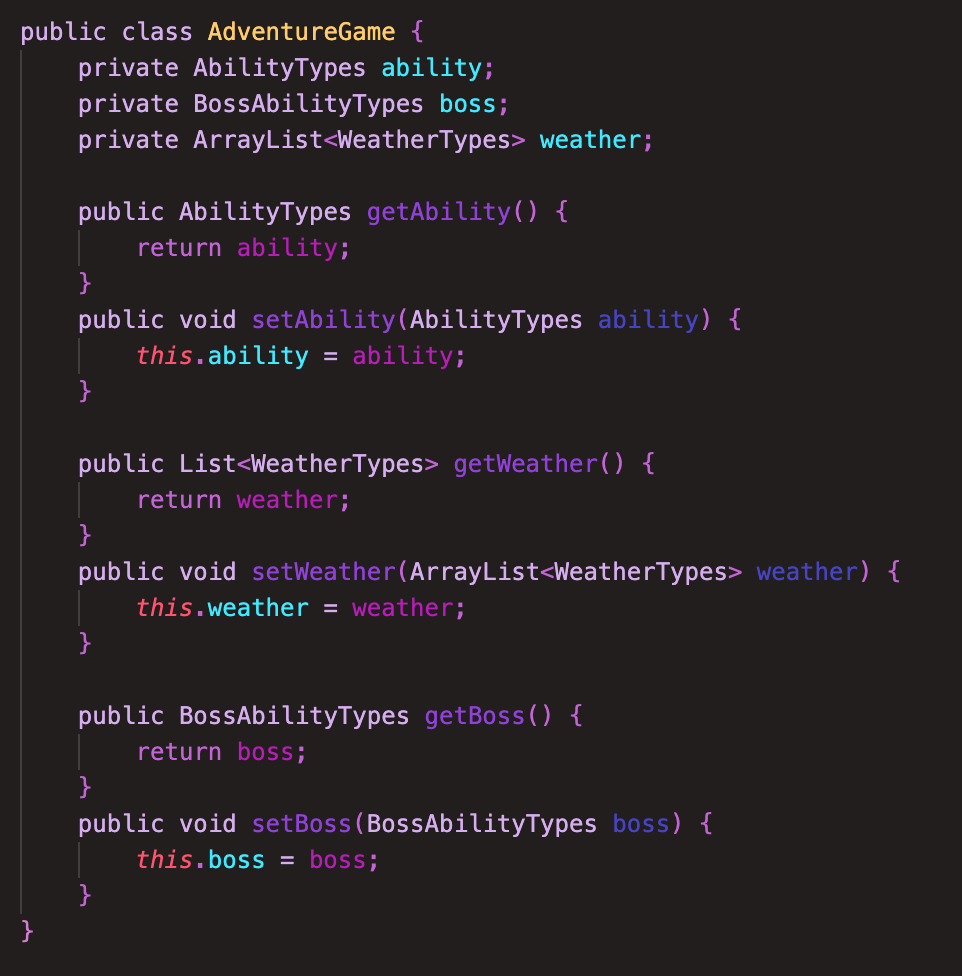
\includegraphics[width=\linewidth]{Materials/Adventuregame/AdventureGame}
	\caption{Super class for adventure games which allows concrete implementations for different variations.}
	\label{MetalanguageAdventure}
\end{wrapfigure} 

To this, we have created a Java class called \textit{AdventureGame} which has methods for setting and getting the player ability, the boss ability and the weather effects. The class can be seen in \autoref{MetalanguageAdventure}. We can inherit from this class to create concrete classes which resemble different variations of our adventure game. We have created several enumerations to hold the possible values for player abilities, boss abilities and weather effects. In \autoref{ConcreteVariation} we can see a variation where the player has the roar ability, the boss has the heal ability and the possible weather effects are blizzard, sunny and cloudy. Only having three different weather effects means that we should only be able to meet these three kinds of weather effects in the game variation, and thus when we talked about randomly selecting a weather type from a pool of available weather effects, we would be able to choose these three weather effects in this variation. Writing the variations in a metalanguage allows to change big parts of the adventure game by writing very few lines of code, making it a very effective way of programming if the code repository for the task is already written.
\begin{figure}[H]
	\centering
	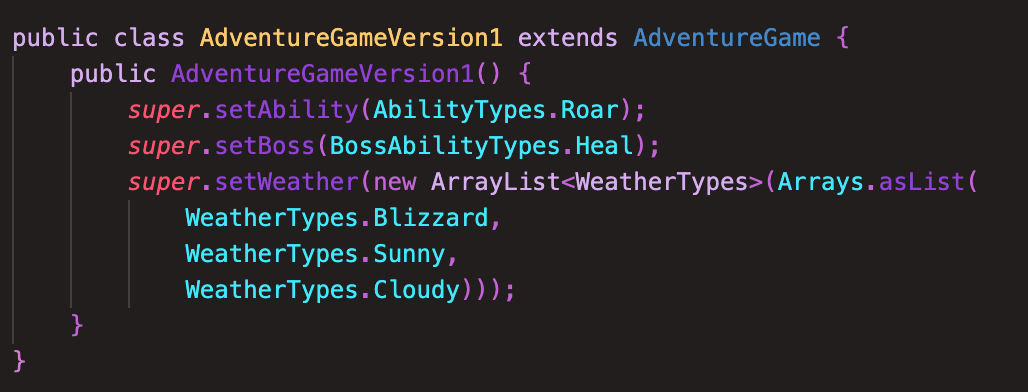
\includegraphics[width=0.8\textwidth]{Materials/Adventuregame/Version1}
	\caption{Concrete implementation of an \textit{AdventureGame}.}
	\label{ConcreteVariation}
\end{figure}

In general the term \textit{metaprogramming} refers to the discipline of writing code which writes code. We here write the Java classes which then with the help of the CLS tool writes the C\# code needed for our adventure game. With the CLS we attach semantic information to each of our combinators such that we with fine granularity can choose the code parts we need. This is a clever way to distinguish code parts which might otherwise just be represented as strings. One could imagine a future where big repositories are created with all sorts of general code and a metalanguage can then be used to speed up development time due to the code already being written, it just needs to be found by a tool like the CLS and be put to use \todo{Keep this part?}. 

\section{Building a repository} \label{BuildRep}
We have already seen an overview of what has been created, but we will now go into details about how we got here. As already discussed in the actor model section '\nameref{AMRelation}' our driving force for the project has been to examine four cases relating the actor model to the CLS, namely:
\begin{enumerate}
	\item Synthesizing objects with timers. This was primarily aimed to be accomplished in the player object through the use of different abilities.
	\item Disposing timers. As both the monsters and the boss have recurring timers and they both can be killed, it is important that we ensure their timers are disposed correctly. If not we might end up with 'invisible' enemies hitting players throughout their adventure.
	\item Synthesizing an object which spawns actors. This is accomplished in the boss with its baseline ability to spawn small monsters in the room with it.
	\item Handling a list of arguments in our meta language. We see this in the weather effects in the rooms where a random weather effect from a given list can be chosen and will have an effect on the players each time they change room.
\end{enumerate}
Our overall goal with this project has been to examine if it is possible to synthesize actor code with the use of the CLS and we found that the four cases above would not be comprehensive but we see the first three to be common tasks performed when coding with the actor model, and the last we foresee to be a common way to program with meta languages when using the CLS. We therefore see the four cases as a good indication of whether it is possible to synthesize actor code on a larger scale rather than a definitive answer to the CLS being a perfect tool to synthesize actor code.\\

Throughout development we found that the coupling between the oldest objects we coded and the newest grew bigger and bigger. This is a tendency we think is rather common in software development (and perhaps also logically) if developers are not careful about their designs and encapsulation. This might also have been an indication that we should have taken a step back and tried to modularize our code more than we have. The fact that the coupling grew with each addition of features made decomposition harder, and finding meaningful decompositions hard as we might just have wanted to change a few lines of code somewhere\todo{rephrase?}. In this rather small project we have managed to work around the coupling, at least to a satisfying extent. However, this might not be the case in bigger projects, and thus our first point to stress is that actors should truly be isolated to allow for good decomposition. To achieve clean repositories we need close to no coupling between objects, and thus good design of programs are essential for decomposition. \todo{Point for conclusion here.}

\subsection{Player} \label{BuildPlayer}
\begin{wrapfigure}{L}{0.55\linewidth}
	\vspace{-10px}
	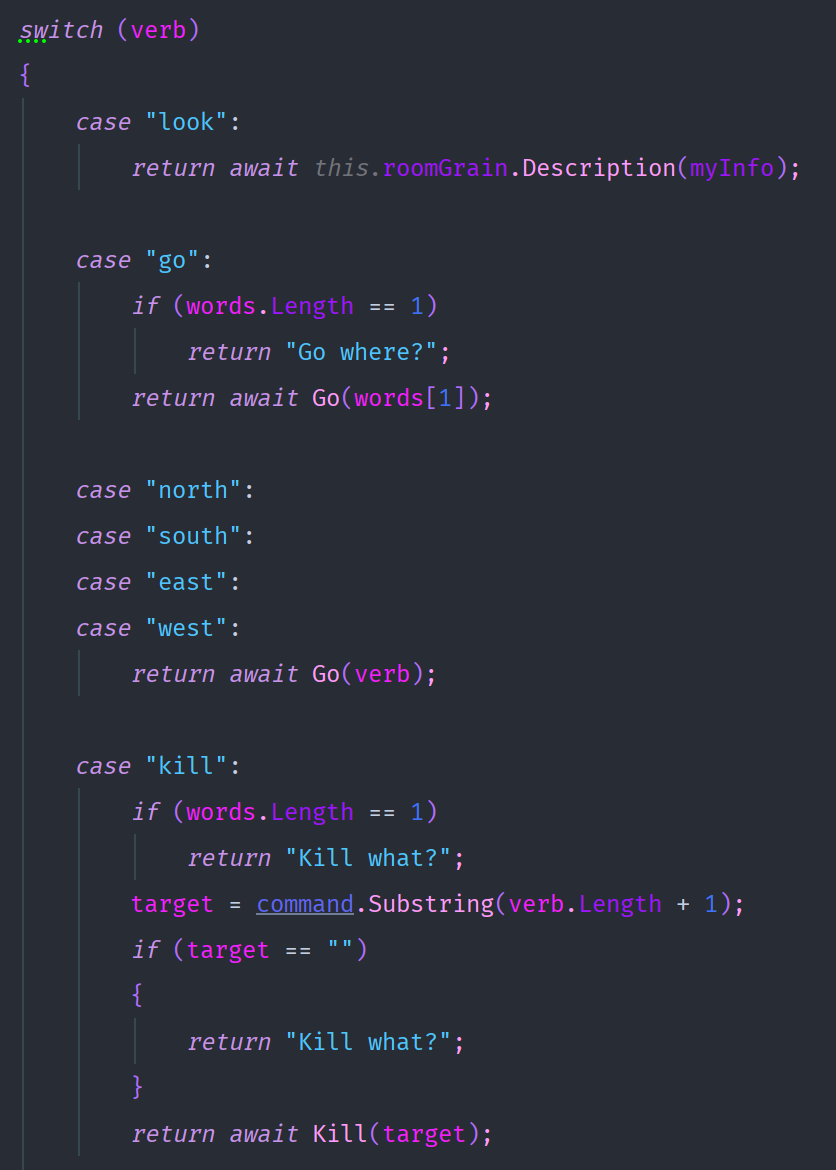
\includegraphics[width=\linewidth]{Materials/Decomposition/switchcases}
	\caption{Part of the switch case in player showing how some actions are implemented.}
\end{wrapfigure}
The player was the first object we implemented and the first we combinated. To understand how we chose to decompose the player we will first look at what makes a player. The player is implemented with a switch case with a case for all the actions the player can take. If we want to move to a new room we could for instance use the command 'go' followed by the direction we want to move. We can semantically look at the switch case as our 'case' or 'cases'.\\
A big part of what makes a player is the abilities it can use. For our implementation we have three variations of what abilities a player can use: fireball, roar or none. As already mentioned \todo{Reference our implementation} does the fireball and roar fulfil two different purposes. The fireball deals damage, and the roar makes the player take less damage. This left us with a choice of either accepting that we would need more information in the form of an extra combinator to ensure that we do not end up with dead code, or to accept the dead code, but making modularization  easier.\\
In our first iteration of the player we wanted to avoid the dead code. This made it hard to modularize the concept of an ability. The fireball simply calls the enemy's take damage function with a higher damage value than the player's standard attack. On the other hand, the roar ability sets a flag in the player which ensures when an enemy attacks, another branch is taken in the player's \textit{TakeDamage} method. The method can be seen in \autoref{PlayerTakeDamage}. To avoid dead code we added more semantic information when we created our repository. Two combinators which provided code with semantic type \textit{'damageTaken'} were thus made. The first having an implementation which did not use the field \textit{'roarActive'} and only had a single line for taking damage, and the second having the full if statement as seen in \autoref{PlayerTakeDamage}.

\begin{figure}[H]
	\centering
	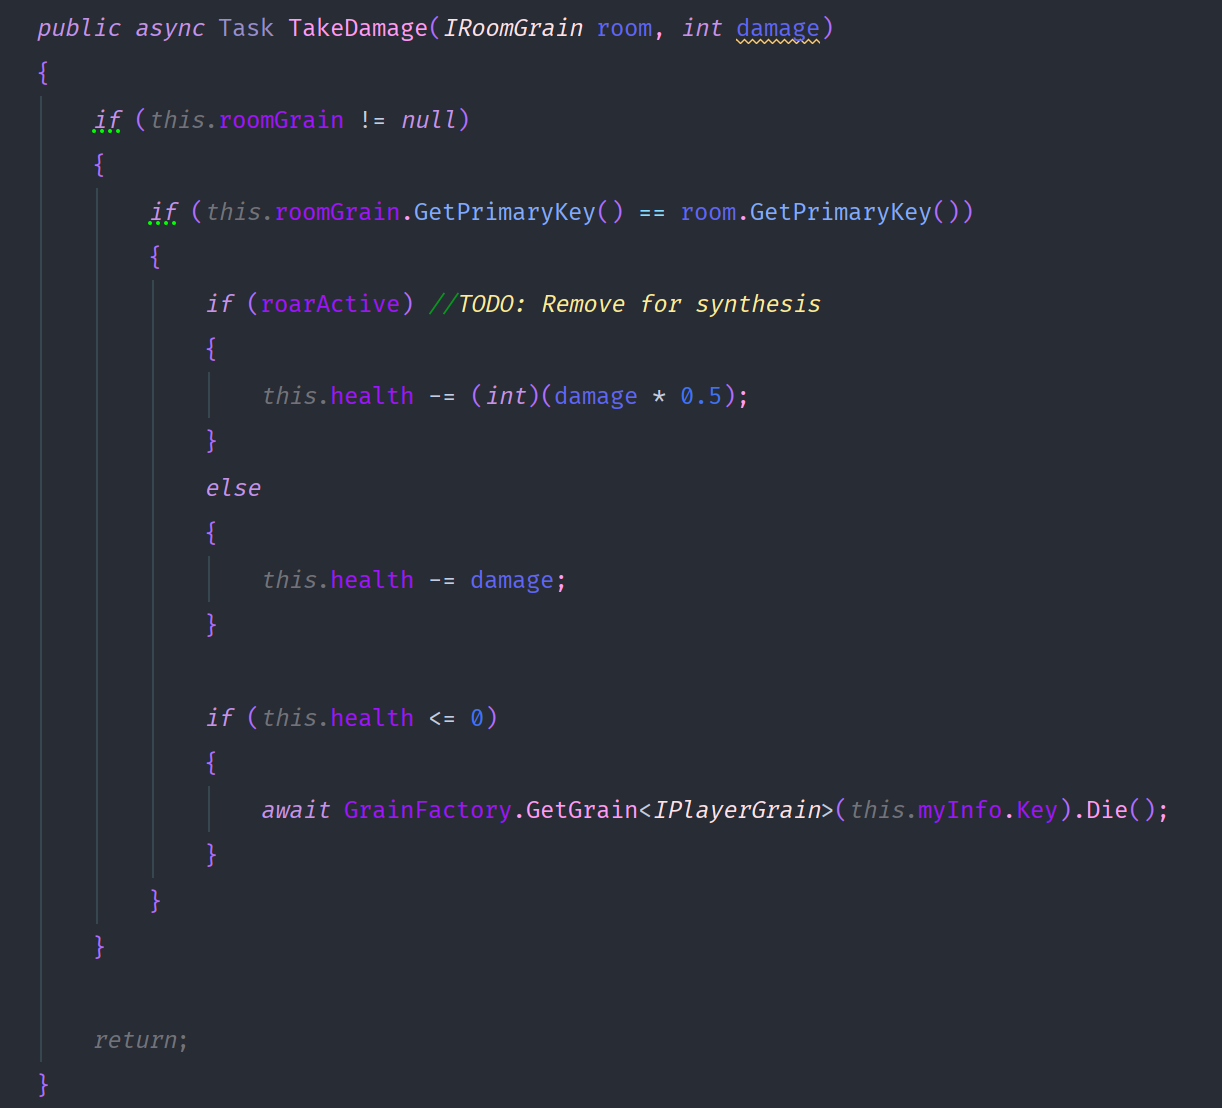
\includegraphics[width=0.8\linewidth]{Materials/Decomposition/TakeDamage}
	\caption{The player's TakeDamage method. Note the if case for when the roar ability is active. Having this if statement means we either need more combinators to describe the synthesis we want, or we have to accept we have dead code. }
	\label{PlayerTakeDamage}
\end{figure}
One can now ask, why is it important not to have dead code? Having dead code means we have fragments of other variations in the code. This means we suddenly have code that does not necessarily makes sense in the current context. A consequence of this could be that we try to access an object that does not exist, making the whole program crash. In general we risk unexpected behaviour which in worst case leads to a crash. This can however be mitigated through thorough testing, showing that it is at least not immediately apparent how the code will show unexpected behaviour based on the dead code \todo{Do we agree that's how testing works?}.\\
On the concrete example of \textit{'TakeDamage'} we see that \textit{'roarActive'} has to be true for the player to take half damage. Designing the player such that the only time this field is set to true is in the roar ability, it would be rather safe to leave the if statement in, as it should not ever be reachable this way. This also made the argument for choosing to leave the dead code and simplify modularization of abilities. However, as we ran out of development time we have not been able to refactor the old code. It could however easily be refactored such that we used dependency injection to give the player an ability which would be its own object with a \textit{'useAbility'} method allowing the player object to call this whenever it needs. The fireball implementation would then call the enemy's \textit{'kill'} method with a high damage value, and the roar implementation would set \textit{'roarActive'} in the player.\\ \todo{Stating we are not going to change player implementation.}
One could argue that in traditional software development it would not be possible to leave dead code in the implementation as we argue in the above that we can, and thus the above is not truly a modularization of the player. To that it could be argued that creating the combinators using the semantic type \textit{'damageTaken} opens up for possible extensions. If there had to be made combinators for how the player takes damage, we have effectively unified what caused the original problem, that an ability both could deal damage and affect how the player takes damage. The only problem here is how we carry this information and rather poor scaleability. Before getting into that we will summarize on the semantics that makes a player.\\
In our concrete implementation the semantics of a player is split in three parts, its actions, its ability and how it takes damage. As already discussed, we have the switch case of actions a player can take and to be able to perform an ability a case needs to be added here. Semantically we can call this a \textit{'case'}. Not surprisingly we can relate the players ability to the semantic type \textit{'ability'}. Lastly we will refer to how the player takes damage with the semantic type \textit{'damageTaken'}. We can thus describe a player as: \textit{string $\cap$ case, string $\cap$ ability, string $\cap$ damageTaken $\to$ MyResult $\cap$ player}. \todo{Unsure if this is a way to long explanation just to reach this rather anticlimactic point?}

\begin{figure}[H]
	\centering
	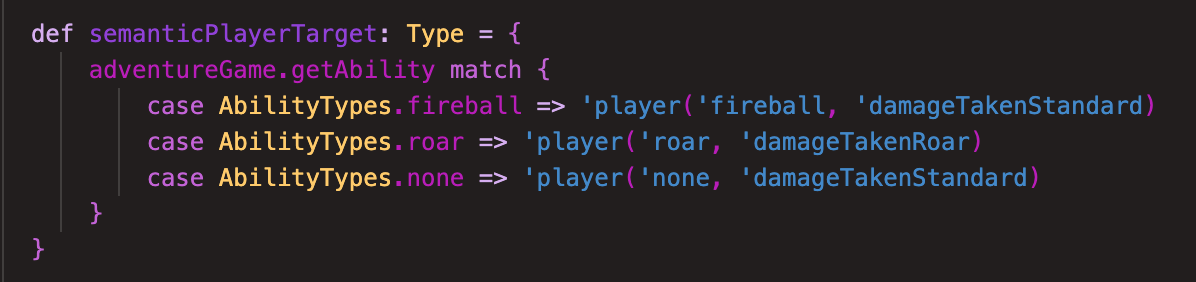
\includegraphics[width=0.9\linewidth]{Materials/Decomposition/SemanticTargetPlayer}
	\caption{The function determining what semantic types in the player we are looking for in our variations.}
	\label{SemanticTargetPlayer}
\end{figure}
So why did we say this approach would scale poorly? This is due to how we carry the information about which variation we want to synthesize. To this we are using \textit{kinding} which allows us to specific about our semantic types. As seen in \autoref{SemanticTargetPlayer} we can for instance have a semantic type \textit{'player('fireball, 'standardDamageTaken}. Here the types \textit{fireball} and \textit{damageTakenStandard} are kindings of respectively \textit{ability} and \textit{damageTaken}. The semantic types (of the same names) can now take these kindings and that way we create the variation we want. For the player the semantic type \textit{'case'} takes the same kinding as the semantic type \textit{'ability'} and that way we always get the corresponding ability to a case. But as we already have noted a player takes two kindings. This is the reason this approach does not scale. If we for each ability have to create combinators and create kindings to carry information forward it will not be feasible to write out all the possible outcomes when appending to the \textit{'semanticPlayerTarget'} function (seen in \autoref{SemanticTargetPlayer}).\\
We previously discussed how we could avoid using the semantic type \textit{'damageTaken'} and obtain more modularization by accepting dead code. Using this approach we can describe a player as: \textit{string $\cap$ case, string $\cap$ ability $\to$ MyResult $\cap$ player}. This approach would avoid introducing more kindings than \textit{ability} and would thus seem more scaleable. However, tweaking the damage reduction for the player would seem problematic but adding other ways to deal damage and adding abilities with different 'purpose' than dealing damage and reducing it would also seem easily done.\\

The player fulfilled the purpose of being an entity with timers. When synthesising the abilities we also include code for timers for the two possible abilities. We can thus say that we successfully can synthesize actor code which uses timers. However, these timers are very simple. They do not require disposing as the player only seizes to exist when the program is closed. Further, these timers are never recurring, so they only fire when the player asks them to. This essentially means that our only consideration with timers for the player is the abilities cool downs (the time before we can use the ability again, because being able to use the abilities repeatedly would make the player way too strong).  
\subsection{Monster and Boss}
The monsters in the game are unsynthesized entities which serve to make the game harder for the player. At their core they can attack the player and take damage. These two properties are shared with the boss, and is thus put in the \textit{IEnemy} interface. Both \textit{IMonster} and \textit{IBoss} implements the \textit{IEnemy} interface, and thus have the core functionality of an enemy. The monsters are interesting to us because they have to dispose their timers. If the timers are not disposed the monster will keep hitting the player after it has died although it would not seem to be in the room with the player. From the monster we can observe it is never the case that they become 'ghosts'. This can of course be explained with the fact that they are unsynthesized, so they always behave the same way. But we also note that the only time the monsters 'exit the game' is when they die, and this is also the time where they dispose their timers. The branch in the monsters \textit{Kill} method where they reach zero health is responsible for disposing the timers, and it is the only 'path' a monster can take to leave the game. The monster's \textit{Kill} method can be seen in \autoref{MonsterKill}. This is thus a very crucial part of the lifecycle for the monsters, one we do not want variations of. We thus observe that a safe way of ensuring a crucial part of the program is always there and always reachable is to make it unsynthesized.\\
The boss always spawn other actors, namely small monsters. This is done on a timer together with its other ability. It is thus also crucial for the boss to be able to dispose its timers. However, this time the entity we are working with \textit{is} synthesized, but the same concerns about always reaching specific parts of code is still present. To solve the timer disposing issue for the boss we used our observation about the monsters, and we decided that only one variation of the \textit{Kill} method should be created. This way we would always experience the same behaviour when the boss dies. The two \textit{Kill} methods are thus \textit{very} similar with small changes to what timers to dispose and what names to return from the call. Although, we do note that there is dead code in the boss' \textit{Kill} method due to the synthesis of one of two abilities. This is however a minor inconvenience as the field with the reference to the ability which is not synthesized is initialized to null, and the timer is only disposed if the field is not null.
\begin{figure}
	\centering
	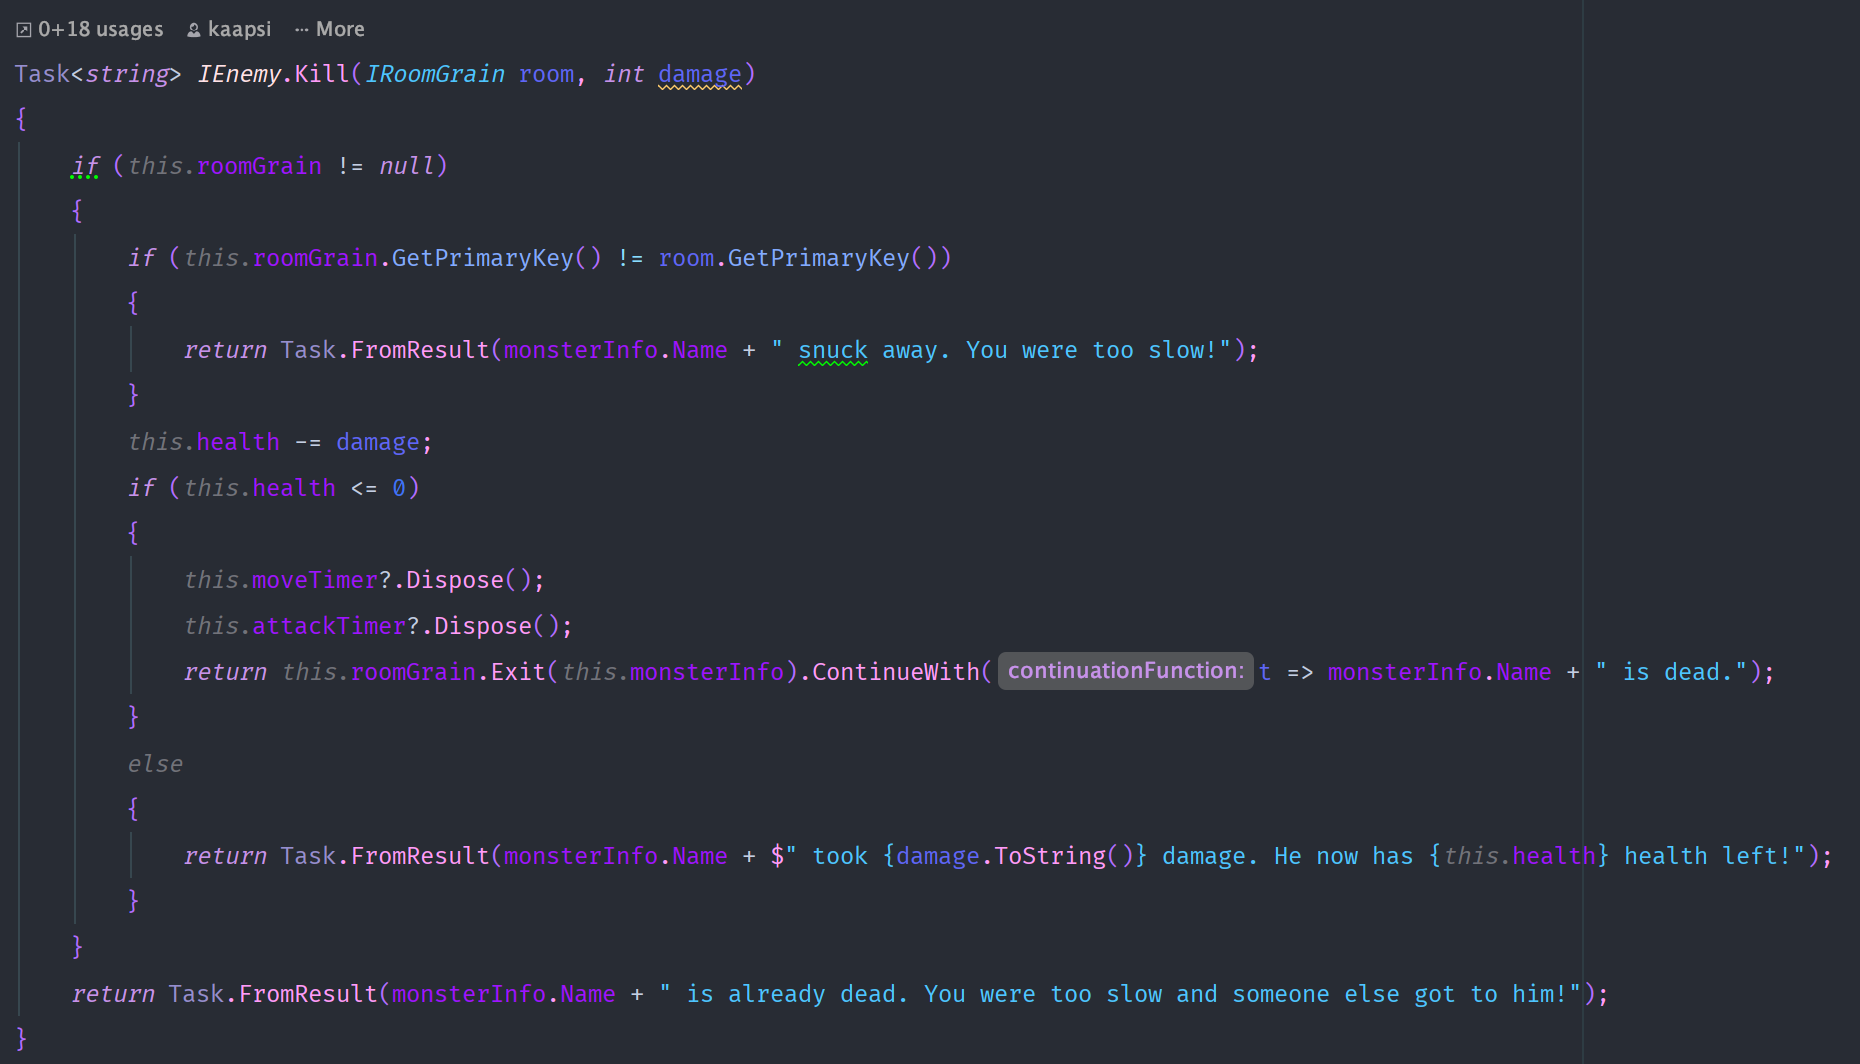
\includegraphics[width=\linewidth]{Materials/Decomposition/Boss/MonsterKill}
	\caption{The monster's method for taking damage.}
	\label{MonsterKill}
\end{figure}

\newpage

\begin{wrapfigure}{R}{0.55\linewidth}
	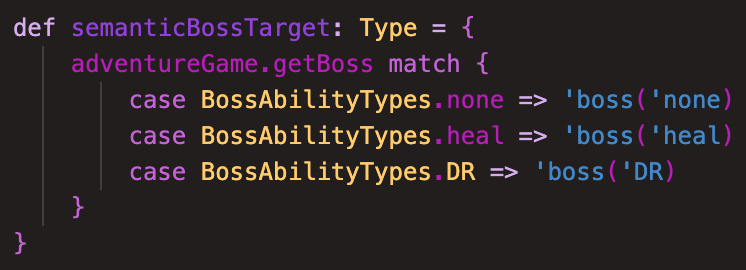
\includegraphics[width=\linewidth]{Materials/Decomposition/Boss/SemanticTarget}
	\caption{Depending on which ability is specified in the metalanguage, we will be looking for different intersections for the boss type.}
	\label{SemanticTargetExample}
\end{wrapfigure}
We found that the boss was a three-part entity, and is defined by its \textit{OnActivateAsync} method, its interaction with the room and perhaps most obviously its ability. We have named the semantic types for each part \textit{'bossOnActivateAsync'}, \textit{'bossRoomInteraction'} and \textit{'bossAbility'} respectively. All the semantic types are intersected by the kinding \textit{'bossAbility'} which can be either \textit{'heal'} or \textit{'DR'} (damage reduction). In our metalanguage we have defined a boss field which can take one of three enum values: \textit{'heal'}, \textit{'DR'} or \textit{'none'}. In \autoref{MetalanguageSetBoss} we see how we can set the boss to have the damage reduction ability in the metalanguage. In our semantic target we match our metalanguage defined boss field with the enum values and get the semantic type \textit{'boss'} intersected by the matching enum type as seen in \autoref{SemanticTargetExample}.
\begin{figure}[H]
	\centering
	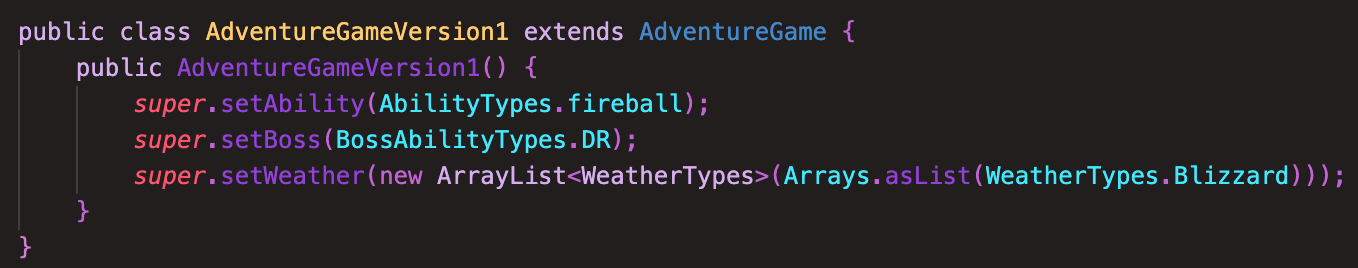
\includegraphics[width=0.95\textwidth]{Materials/Decomposition/Boss/MetalanguageSetBoss}
	\caption{Here we see how the boss is set to have the damage reduction ability in the metalanguage.}
	\label{MetalanguageSetBoss}
\end{figure}

For the semantic type \textit{'bossOnActivateAsync'} we have two combinators, one where the timer for the monster healing ability is started, and one where it is not. Otherwise there is a small additional setup for the boss which is the same for both combinators.\\
The two combinators for the abilities are also very simple. The variation with the heal ability implements the \textit{HealAdds} method whereas the variation with damage reduction is just an empty string. This is because there is no method for the damage reduction, its just a flag which is set whenever the boss spawns a new add.\\
This leaves us with the interaction between the room and the boss. To remove the damage reduction from the boss it needs to know when the adds die. For this we have added an observer like pattern between the room's \textit{Exit} method and the boss. Usually when implementing the observer pattern, several objects wants to know that something has changed in a single object, and so the single object broadcasts that this change has happened rather than the many objects asking \textit{if} there have been a change. Here the room knows when the adds dies, namely when the \textit{Exit} method is called. We thus changed the \textit{Exit} method to call the boss' \textit{UpdateAdds} method. This is obviously dead code in the variations where we do not have any boss, and so we make a check for the boss being present in the room. The semantic type \textit{'bossRoomInteraction'} include the \textit{UpdateAdds} as it is here we set the damage reduction flag back to false, but it also includes the \textit{SpawnAdds} method as it is here we set the flag to true. Given \textit{SpawnAdds} calls the room's \textit{Enter} function (and thus has an interaction with the room) for the newly created monster, we thought it would be fine to include both methods in the same combinator instead of creating more types and more complexity.\\
We here notice somewhat the same issue as with the player's abilities, namely that they do not share the same purpose. We see that the two abilities only changes a single line in \textit{SpawnAdds} and only a few lines in \textit{UpdateAdds} where the damage reduction flag is set. At first, one would think we could use dependency injection to define a common interface for boss abilities. But this would require the statement which sets the damage reduction flag in \textit{SpawnAdds} to be replaced by a call to an ability use, which would execute the healing ability each time an add is spawned which is not what we want. We here notice that the healing ability is on a timer whereas the damage reduction has a more event driven behaviour as it triggers when an add is spawned and when an add is killed, and the 'nature' of the two abilities are thus different. Using dependency injection would require one of the abilities to change 'nature' as either we would need to heal every time an add is spawned, or we would need to provide damage reduction on a timer. Changing the damage reduction to be on a timer which aligns with the timer for \textit{SpawnAdds} could work as it would remove the one-liner from \textit{SpawnAdds}, but we remove the synchronization of the damage reduction and the add spawning, and risk that an attack hits the boss between the add spawn and the damage reduction. We found that our implementation is the best solution to the issue although it to some extent limits the extendability of the boss.\todo{måske noget visualisering?}\\
For the variations with no boss we created a combinator which requires nothing, but creates a semantic type of \textit{'boss} intersected with \textit{'none} where the boss grain is simply empty.\\

One might now ask, how do we spawn the boss? This is done in \textit{'Adventure.cs'} where we add the method \textit{AddBoss}. This of course would also have to be synthesized and so if a boss is set in our metalanguage we have a combinator with our changes added, and if we are having a variation without a boss we have a combinator without our changes. We tried to merge this synthesis with the boss, but due to the limitation of only being able to create one file per job added to the CLS we had to split the synthesis in two.\\

In conclusion we found that the best way to ensure disposal of timers is to make it the only 'path' possible. We did this by only having one way for the monsters and the boss to exit the game, and that involved disposing their timers first. For safety we decided this was best done in unsynthesized code as this would ensure uniform behaviour no matter what variation we create.\\
We also see that spawning additional actors is no problem in a synthesized setting, and this can easily be achieved on a timer as with the boss. The only problem we encounter is created by us, and is how we have weaved the damage reduction ability into the add spawning. Although this approach to us seems better than the alternatives, it still limits the extendability of the boss.
\subsection{Room}\label{Room}
The rooms are central parts of our game as they hold the information about who is where and can be seen as the glue which keeps everything together. Our overall goal has been to be able to define a list of weathers for which we can then synthesize rooms which has these chosen weathers. In the meta language we can for instance define a list consisting of \textit{blizzard} and \textit{sunny}, and so the only two weather types which should be encountered in this variation are \textit{blizzard} and \textit{sunny}. We created in total four different weather effects, \textit{blizzard, sunny, night} and \textit{cloudy}. To make the room able to use different weathers we followed a strategy pattern where each weather type conforms to the \textit{IWeatherEffect} interface. Every time a player enters a room it will at random choose a weather effect from the defined possibilities, and its \textit{WeatherEffect} method is called. This way the room can conform to many different strategies as to how the weather should effect the player. \\
We found that what makes a room is what weather types it should be able to use and whether there is a boss in the variation or not. Each of the weather effects have their own kinding which allows the to be either the weather or \textit{'none}. Given all weather type kindings has the type \textit{'none} in common, we only have to create a single combinator for this option as they can all share it. We can attempt to be a little more concrete by looking only at the semantic types in the following. We are looking for room. As mentioned this is defined by the weathers and whether there is a boss present or not. And so we are looking for: \textit{'bossActive(boss), 'weatherTypes(blizzardWeather, sunnyWeather, nightWeather, cloudyWeather) $\to$ room(blizzardWeather, sunnyWeather, nightWeather, cloudyWeather, boss)}. We read this as we need something of semantic type \textit{'bossActive} intersected by the kinding \textit{boss} and we need something of semantic type \textit{weatherTypes} intersected by the weather kindings to get something of semantic type \textit{'room} intersected by the weather type and boss kindings. The boss part is fairly straightforward as either there is a boss or not. The kinding is reused from the player and the combinator for when the boss is present consists of three methods which are added to the room, whereas if the boss is not present, the combinator is an empty string. The two combinators for \textit{'weatherTypes} are more complex. We have two as the code needed for having no weather effects and having one or more weathers are quite distinct.

\begin{figure}[H]
	\centering
	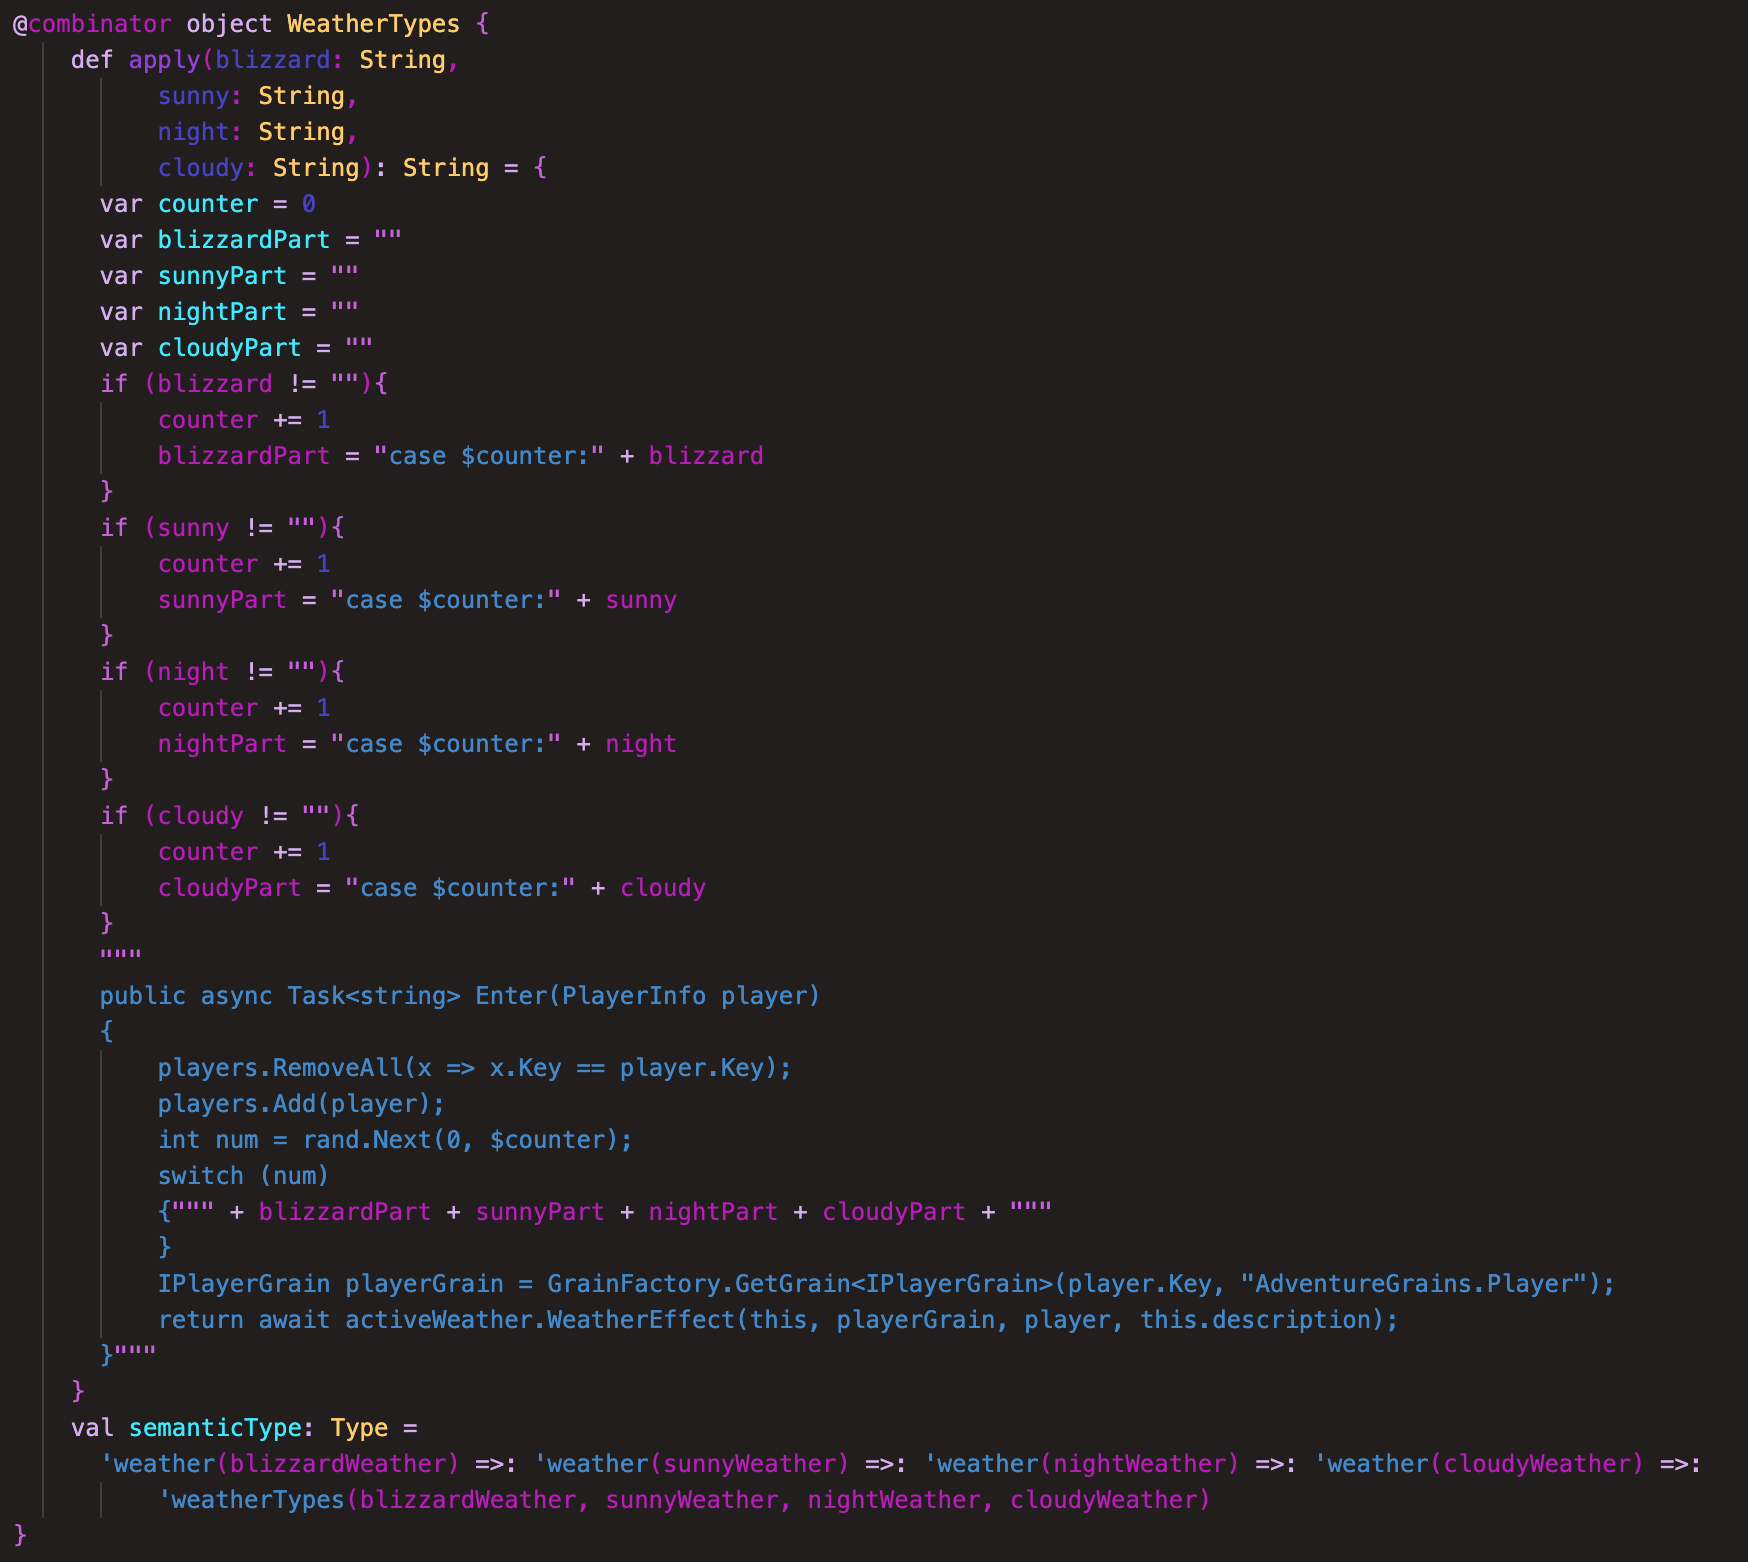
\includegraphics[width=\linewidth]{Materials/Decomposition/Room/WeatherEffects}
	\caption{The combinator used to create variations with weather effects.}
	\label{WeatherEffects}
\end{figure}
In \autoref{WeatherEffects} we see the combinator for creating weather effects. As it is not trivial how this combinator works we will go a little more into detail about how it works. The overall structure we are working towards is a switch case where we at random will choose what weather effect the player should experience. We see that we need four \textit{'weather} types, one for each possible weather effect. These come from simple combinators providing two lines of code for the \textit{WeatherTypes} combinator. We then check each of the weathers if they should be present by checking whether the string provided to \textit{WeatherTypes} is empty or not. If it is not empty, the code provided it appended to "case " and then the number of a counter. If two weathers are present, the first will then be of case 0, and the second of case 1. After we have created the cases for each of the weathers present, we then insert them in the 'static' part of the combinator as part of the switch statement. We note that this combinator ends by calling a weather effects \textit{WeatherEffect} method. All the weathers call the room's \textit{Description} method which is the biggest change when looking at the combinator used when we do not have any weather effects, as now the room has to make this call itself. The combinator for no weather effects can be seen in \autoref{NoneWeather}.

\begin{figure}[H]
	\centering
	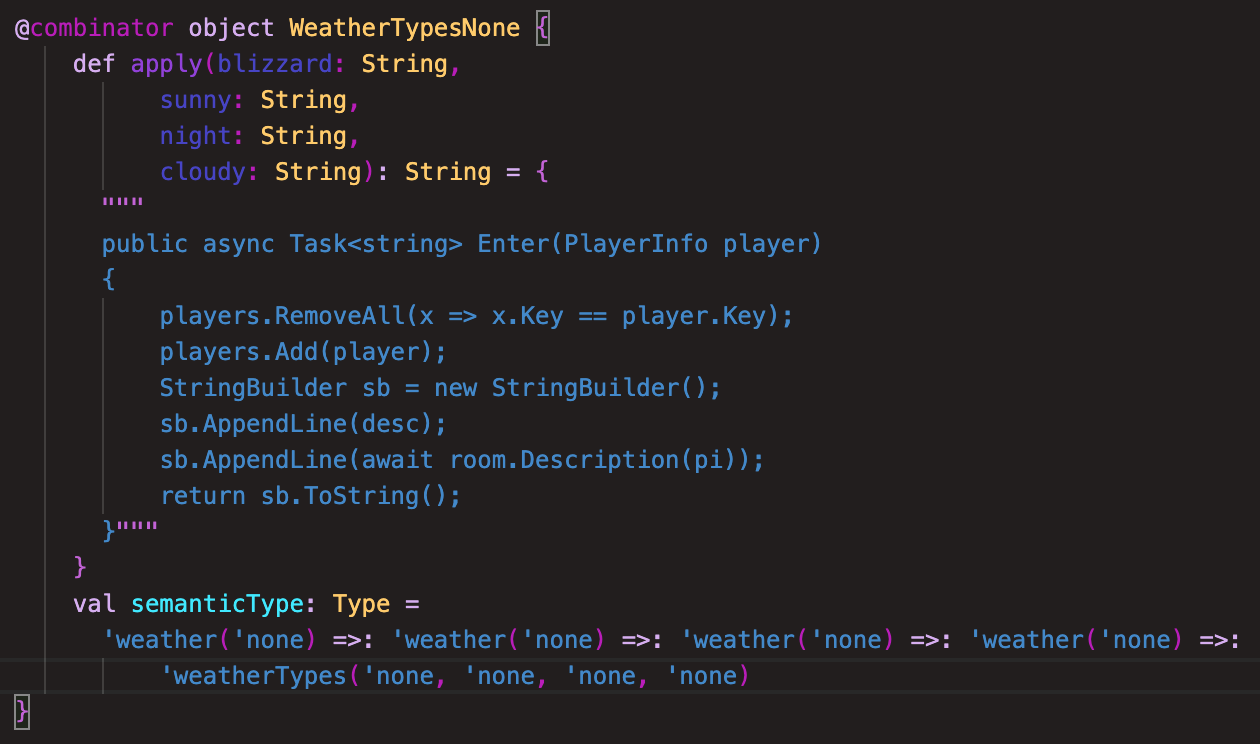
\includegraphics[width=\linewidth]{Materials/Decomposition/Room/NoneWeather}
	\caption{The combinator used to when we do not want weather effects.}
	\label{NoneWeather}
\end{figure}
Unfortunately we see that when we create a variation with no weather effects we will get two variations. This is because both combinators accepts four \textit{'weather} types intersected by \textit{'none}. We could avoid this issue by intersecting \textit{'room} further. For instance adding a kinding \textit{'weatherPresent'} which can take the values \textit{'weatherIsPresent} and \textit{'weatherIsNotPresent}. We could then add a combinator which provides the first few lines which \textit{WeatherTypes} and \textit{WeatherTypesNone} has in common and has the semantic type \textit{weatherEffect(weatherPresent)}. \textit{WeatherTypes} would then require \textit{weatherEffect(weatherIsPresent)} and \textit{WeatherTypesNone} would require \textit{weatherEffect(weatherIsNotPresent)}. Then the \textit{weatherPresent} kinding would be set in the \textit{SemanticRoomTarget} method depending on whether all weather kindings are \textit{'none} or not. This is however, a lot of additional complexity and begs the question, is creating a combinator for the first few common lines of code meaningful? The consequence of not doing this, is the developer needs to choose the correct variation of the room, which we do not see as a huge issue. And we thus value the simpler solution more, as we see the added complexity to do more harm than having to choose between two variations do. However, this is a small project, and in a bigger setting it might be better to choose the alternative solution as it is more scalable.\\

Although we were very confident we could combinate these weather effects, we have unfortunately not been able to do so. We are unsure what exactly the problem is, but when attempting to create a variation based on \textit{SemanticRoomTarget} the CLS will run for one to three hours before throwing an 'out of memory' error. This indicates there is a loop in the code somewhere, but despite our best efforts to debug the code, we cannot find the error. As so, we conclude that we have not achieved our goal of being able to synthesize code where a list of parameters defined in our meta language has an effect on the variation we are creating.


\subsection{Good decomposition}
One can now raise the question, did we achieve good decomposition? To answer that, we would need to look at what makes a good component. This has been a difficult task to answer, as it has been hard to find literature that answers that question. The closest we have got is \cite{Components}, but the focus can be seen to be on a bit higher level than our decomposition. \cite{Components} gives the impression that a component is a collection of code wrapped in a well defined and well documented interface. The focus is on how the component will be communicating with the other classes of the system through its interface, and so there is great emphasis on the design. We can look at this from two angles. We can look at our components as the actors of our system, the player, room, monsters and boss. Here we see encapsulated units with some dependencies on each other and well defined interfaces for the interaction they have with each other. We here have some units which could be reused in another game which is structured the same way. However, we can also look at each of the actors and decompose them. It is here it gets a little uglier and many of the issues described in the previous subsections arise. When we decomposed the actors we did not create a standard for what the components should be and thus we did not create interfaces for them. We have already discussed when it would have made sense and when not to use dependency injection, but not using interfaces makes it hard to reuse components in other projects, and so looking at our individual combinators, its not a lot of them that are reusable. We did not really intend each combinator to be reusable by itself as our goal was to combinate the actors. Our goal was to create interesting variations which were not too similar, and we believe that we succeeded there. However, depending on which angle we look at our decomposition, we get different results. Although less coupling and less dependency on the room would be preferable, we still feel our actors are encapsulated and independent. It is hard to keep both the single responsibility principle and have no coupling, and so we feel we have a good trade off. If we look at the system as a whole, the actors becomes some of the components and although some design decisions have made it hard to extend them we see them as decent components, and thus we have achieved somewhat good decomposition.\\
Had our goal been to create the components for our actors, we would probably not have been combinating our actors as a whole, but instead creating smaller classes like a 'PlayerAbility' class which we would then create different methods for. The end goal would be the same, a player with an ability, but here all the combinators would be reusable. It is thus important to distinguish the two viewpoints from each other when we evaluate our decomposition as they yield two very different results. We can however compare the two approaches, and conclude that we have probably chosen the wrong approach due to both simplicity and the amount of combinators which could be made reusable.

\subsection{Future work}
In future work with the CLS and Orleans we cannot put enough emphasis on how important a good solid design is. When we began learning about the CLS we thought it would eliminate the need for dependency injection, we just replace code so why make a socket for it? After working on this project we now understand the importance and we understand that the CLS does not replace any already existing software engineering principles, on the contrary, using the CLS makes it much more important to follow them. Both the CLS and Orleans strive to work with encapsulated and isolated code which has no to little coupling with other entities, and so they both seem and feel to be a great match together, also for future projects.
\section{Testing Theory}
%Integration
%State testing?
Testing is a quality-improvement activity meant for detecting errors in the software you write, meaning error detection, however it may sometimes falsely be referred to as "debugging" \cite{TestingCodeComplete}. Testing is a large topic, that spans way beyond testing during development, meaning it may be in place to specify our scope of testing. \\
We will look and describe the two testing areas that we have performed. While software is tested in a number of ways, we will solely look at unit testing and integration testing. \\%meh
Unit testing is the testing of a single routine, class or small program, in isolation from the rest of the system. This is to ensure that the individual classes and their methods work as intended, without any dependencies\cite{TestingCodeComplete}.
Integration, on the other hand, is testing of two or more routines, classes, etc. After unit testing, we know the individual classes or components work in isolation. Integration testing is the testing of the connection and interaction between the classes, such that we ensure the system works in unison. \\
Unit testing is performed before the integration tests, as to ensure the individual classes work, before testing them all together. If we used integration test first, and a given test failed, we would not know whether the fault was in a specific method or the communication between classes. \\
\subsection{White-box and Black-box Testing}
%basis testing
%control flow
%data flow
%AAA
We usually split testing up into two categories: black-box and white-box testing. Black-box testing refers to tests in which the tester does not have access to the source code and must hence test based on the specifications of the given methods, meaning testing based on what the method is supposed to do, hence the method works as a black-box. White-box testing is the other scenario, where the tester has access to the method. This means that the tester is aware of the control flow and routes the method can take, such that testing can rely on the inner workings of the method instead of only the specifications\cite{TestingCodeComplete}. \\
However, even though we are the developers, we do not have direct access to the code. This is because, while we do have access to the combinators and the pre-synthesised code, we will not be able to see the synthesised code doing our synthesising of our tests as well \todo{Needs rephrasing}. The synthesised code will work as a sort of black-box, since we do not actually know how the code looks like and hence making white-box testing would prove difficult, without analysing our generated files. So with this in mind, we have chosen to focus on black-box testing, as this seems as the more accessible and appropriate path to take. \\
Black-box testing is mainly split up in two parts: Data testing and state testing. Here, data testing refers to the data, meaning the input, while state testing is about the program, that is the flow, transitions, logic, and so on\cite{TestingBlackbox}. Let us look at these two parts more closely, some of the methods to use in these cases\todo{Needs rephrasing}. The two major methods under we will look at are equivalence partitioning and boundary conditions. \todo{Maybe rephrasing?}.
\subsubsection{Equivalence Partitioning}
The most important task when it comes to testing is selecting the right test cases\cite{TestingBlackbox}. After all, if we had a simple program that took an integer as input, we could, theoretically, make infinitely many tests for this. This is where equivalence partitioning, also called equivalence classing, comes in. The idea here is that we reduce the infinite possible sets of test case, while still being as effective. We want to split the data into partitions, such that we can use a single test that counts for a range of possible input. For instance, how different would it be to test for 1, 2 and 3 as input as opposed int.MaxValue? We would expect that the first three cases would act similarly, while the program would have to handle the maximum integer value differently. However, how do we know for sure what input to put in the different partitions? The short answer is we do not. Equivalence partitioning can be subjective, such that different testers may come up with different partition sets\cite{TestingBlackbox}. \todo{mere? edge cases?}
\subsubsection{Boundary Conditions}
Boundary Conditions is about testing the method at the boundaries. As a good illustration of what boundary condition is and is for, you could imagine walking along the edge of a cliff. If you can traverse this part safely, you can most likely traverse away from the edge as well. Meaning, if we can show that our methods work at the edge of their capabilities, chances are they will almost certainly work under normal conditions as well. These boundary conditions, also known as edge cases, are important since with programming, problems are more likely to occur at the edges\cite{TestingBlackbox}. This means that, for instance, if we could input any number between 1-100, it would be better to test the edges, such as 1 and 100 than numbers in the middle. \\
We can combine this with the Equivalence partitioning explained earlier. We could split our testing into two equivalence partitions. One should be the edges, those that we expect to work, meaning in our number example it could be 1 and 100. The other equivalence partition would then be outside the boundaries, meaning cases that could likely cause an error, or some unexpected behaviour. In our example, this could be 0 or -1 and 101, just outside our boundaries. 
\subsubsection{Default, Zero and Blank}
Another thing we can look at is testing our methods with a default value. In this case we mean, for instance, if our TakeDamage() method, is parsed 0, what happens then? Or the play function, which is our player's way to interact with their surroundings in the game, by entering things like "fireball witch", "go north", etc., what happens if we enter the empty string? These types of cases can be classified as forms of edge cases, but they are still important to include, as these situations may have been overlooked during implementation of the methods\cite{TestingBlackbox}.
\subsubsection{AAA}
One last thing we want to look at is the structure of the individual unit tests. Usually they conform to the AAA pattern. AAA stands for arrange, act and assert. Using this form of pattern makes it easy for other people to understand your tests\cite{TestingAdaptiveCode}. \\
The arrangement part is also referred to as the setup. Before we can actually perform a certain test, we need to set up what we need in order to carry out the tests. A simple example would be instantiation of the class to be used in the test. Without instantiating the class, we will not have a valid instance to test. \\
The act part of AAA is the execution of the method to be tested. Optimally, this should only consist of a single interaction, for instance meaning a single method call\cite{TestingCodeComplete}. This ensures that the individual tests are simple and precise. \\
The last part of AAA is the assertion. This is the actual testing part, where we will see whether our act part has performed as expected, or produced another, unforeseen, outcome. \\
\\
However, we have diverged a bit from this concept for two reasons. First off, the testing framework we are using, NUnit, allows setup code to be run from the constructor. This means that the arrange aspect can partially, if not fully, be moved to the constructor of the test class. \\
The other reason is readability and transparency. If we have a test, NUnit allows the ability to run the same code with various data input. This means we can have multiple testcases, under the same test function. At a first glance, this may look better, as there is less code in the function, however, it can make the assert part more unclear. If we want to make multiple testcases of the same test, our expected value had to be dynamic, which would obfuscate what we really intended as the expected value.\todo{Do we use this? Is it relevant?} \\
So instead, we explicitly state what the expected outcome is. 
\begin{figure} %MINDRE?
    \centering
    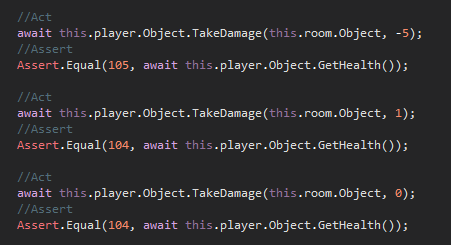
\includegraphics[width=0.8\linewidth]{Materials/TestingTheory/playerTakeDamageAAAtest}
    \caption{Part of the player's DamageTest(), showcasing the AAA structure.}
    \label{playerDamageTest}
\end{figure}
if we look at \autoref{playerDamageTest} we can see how we diverge from the described form of AAA, where our test includes the various testcases with different input, instead of feeding the data to a dynamic test. Here we can also see how we explicitly state the expected outcome for each testcase. 

% As we have been the developers of our product, we will omit black-box testing and focus on white-box testing. As stated, since white-box testing includes the source code, we can more thoroughly test our methods and hence, with white-box testing, cover the same testcases as black-box tests, making them superfluous. \\% måske?
% Now, under white-box testing we have different testing methods to make sure our tests are thorough. Futhermore, there are two aspects we will look at shortly: control-flow testing and data-flow testing. As the name suggests, control-flow testing is about testing the control statements of a method, and making sure we test all possible routes. Data-flow testing is focused on the variation of data and the idea here is that data is atleast as error-prone as control-flow and should therefore be tested as well\cite{TestingCodeComplete}. 

% \subsubsection{Structured Basis Testing}
% We will start by looking at control-flow testing. Here we have structured basis testing, which is a pretty simple concept. We want to make sure that each statement in the given method is run at least once during testing. We can use a simple approach to figuring out how many testcases are needed for basis testing at a minimum, by following these three steps\cite{TestingCodeComplete}:
% \begin{itemize}
%     \item Add a testcase for the method itself.
%     \item Add a testcase for each of the control-flow keywords in the method. (if, while, for, and, etc.)
%     \item Add a testcase for each case in a case statement. Add an additional testcase if the case statement does not include a default case.
% \end{itemize}
% For instance, if we picture a simple method that contained a simple if-statement, we would need two testcases: one for the simple path through the method, and one for the control-flow keyword if. From this we can see that, based on the complexity of the method, the number of testcases we will need to cover all statements increases quickly. \\
% So, with structured basis testing, we assure that all code of a method is executed. However, as mentioned earlier, data-flow is atleast as error-prone, and structured basis testing does not take variation of data into account.

% \subsubsection{Data-flow testing}
% With data-flow testing, we want to ensure that not only all statements are covered, but also all combinations of variables in the code. With structured basis testing, we get a weak form of data-flow testing, since this executes all lines of code, which includes all variables\cite{TestingCodeComplete}. This, in turn, gives us some of the combinations of data, but not them all. We want to extend upon the structured basis testing to include data-flow testing and this calls for more testcases. Here, we want to add all the combinations of variable states that have not been included in the structured basis testing. %Hmmmm
\subsection{Test Doubles}
%Test doubles / isolation
%Moq framework +example
The way our code is written, we have a certain focus on the room, wherein the other actors may reside. This means that a lot of the methods requires a specified room, to know where and what to look for. In short, we have high coupling between our classes. However, in unit testing, we wish to perform tests of each class in isolation, independently of the other classes. So, if we have high coupling, and yet want to test classes independently, how are we to do this? \\ This is where test doubles come in. Using test doubles, also known as scaffolding, is the means of making it easier to isolate code for testing. The point of a test double is to act as a class, including some of its functionality, so that it can be used by another class that is being tested\cite{TestingCodeComplete}. There are various test doubles available, such as fakes, dummies and mocks. Since mocking is what we are going to use, this is what we will look more into.

\subsubsection{Mocking}
The idea of mocking, or mock objects, is to mimic the behaviour of the real class we are imitating. However, we can do this in a controlled way, such that the methods of the mimicked class returns some specific values, independently of the input they receive. This means that the class will not produce any specific results based on their real implementation, but predefined output that we specify\cite{TestingAdaptiveCode}. As such, if we have a class we want to test, that is dependent on the class we mimic, we can now replace the dependency with our mimicked class. Now we have isolated the class we want to test, as all interactions with the mimic is controlled. \\
\\
To mimic the behaviour of a real class it would require us to make a new class. For each class we would like to mimic, we would have to make seperate classes for. This does not only mean that we would need a lot of extra code just for our unit tests, but also that if we were to change the actual class, we would have to change the mimic. This could, potentionally, become tedious work. To get around this, we make use of a framework, that enables us to make the mock objects dynamically, namely the Moq Framework.

\subsubsection{Moq Framework}
This will serve as a short introduction to the Moq framework and how we use it in our testing. \\
We already mentioned how making our mocked versions of the various classes manually would be tedious work. Luckily, the Moq framework makes it easy for us to mock a given class. This framework is very powerful as it allows us to manipulate the behaviour and expectations of our class\cite{TestingAdaptiveCode}. The major part of the mocking lies in the setup. When setting up a new mock, you can specify with the help of the Setup() function, what a given function should return, based on some specific or generic input. Let us take a closer look at the first line of the function body in \autoref{TakeTestMoq}. 
\begin{figure}
    \centering
    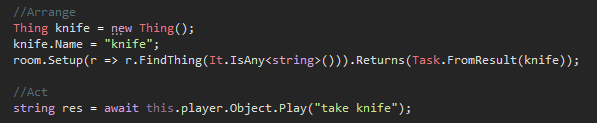
\includegraphics[width=0.9\linewidth]{Materials/TestingTheory/testTakeTestMoqExample}
    \caption{Part of player's TakeTest() showcasing the moq framework's setup}
    \label{TakeTestMoq}
\end{figure}
Here, we can see a nice example of the moq framework. The variable here, room, is of Mock<IRoomGrain>. As we can see with the lambda function, we specify that by a call to the room's FindThing() function, with an input of type string should return the newly created knife. This way, we can test the player's take command, that requires the room we are currently in, as well the items in this room, without the interaction of an actual room. This ensures that we can test the player in isolation, while also noting that the player indeed does send a message to the room grain. It should also be noted here, that while player is of type Mock<PlayerGrain>, by calling player.Object we effectively have the mocked player of type IPlayerGrain and not a player of type Mock<PlayerGrain>.

\subsubsection{Mocking a Class vs Mocking an Interface}
We would also like to shortly explain the difference between mocking a class and mocking an interface. As is made apparent in our tests, we mock both the class under testing and the classes that it depends on. The only difference in the mocking between these two is that the class under testing is a mock of the actual class, while its dependencies are mocks of their interfaces. \\
Mocking an interface creates an instance of the class that implements this interface, but with no actual implementation or logic. For instance, if we look at \autoref{TakeTestMoq}, we set the room's FindThing() function to return a knife to us. If we did not do this setup, the function would not have been implemented and given us and error instead. \todo{er det hvad den gør?} \\
Mocking a class creates an inherited class of the mocked one, which per standard uses the base implementation of their functions. So if we mock a class and make no setup, the functions will be the same. However, the smart thing about mocking these classes for testing, that function virtually the same as the original class, is that it allows us to change certain behaviour, while still maintaining the same functionality, such that we can test it properly. \todo{cite} \\
We will look more into why this is important, and how we have changed certain aspects of the code, in the DISCUSSION SECTION GRAINFACTORY. \todo{reference}

%Gem GrainFactory for discussion
% \begin{figure}
%     \centering
%     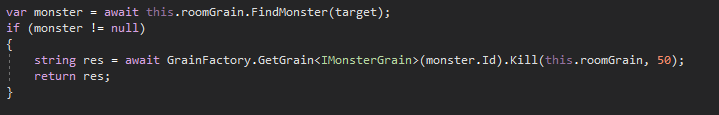
\includegraphics[width=\linewidth]{Materials/TestingTheory/FireballGrainFactory}
%     \caption{Snippet of player's Fireball() function, showcasing the problem with GrainFactory. Even if our room was mocked and returned our mocked monster's id, GrainFactory would create a real monster based on this id, as it finds no monsters with this id.}
%     \label{fireballGrainFactory}
% \end{figure}
% However, we do still have a problem, since this mocking does not cover all of our coupling of the grains. We can access different grains by calling GrainFactory.GetGrain<Type>(id), but by the nature of grains, if we call this function, with an id that does not correspond to any existing grain, it will automatically generate one for us. These methods are called inside some of the different functions of our grains, meaning that even though we can mock a monster, if a function inside player calls a function inside monster through the use of GrainFactory, it will ignore any mock monster we have created and make a real IMonsterGrain for us instead. We can see this problem illustrated in \autoref{fireballGrainFactory}. \todo{Måske cite + billede er godt til at illustrere?} So, how do we get around this? \\
% One way to side-step this issue is to mock the GrainFactory function of the class we are currently testing. To do this, we have to expose the GrainFactory function of the class, as it normally is a protected function. We would then create an override of the GrainFactory function, which means that we rewrite code in our classes due to our tests and while this is bad practice, it must be done in order to mock the GrainFactory and ensure that our grains do not make their own grains when we want them to use our mocked grains instead \todo{cite?}. \\ 
% This does open yet another issue. The new GrainFactory implementation cannot be part of our interface, such that if we want to use our mocked GrainFactory, we would use mocks of the classes instead of the interfaces (e.g. Mock<PlayerGrain> instead of Mock<IPlayerGrain>), rendering some of the interfaces functions hidden and unsuable for testing. \todo{Billeder? what to do med problemet? "maskintekst" for funktioner i vores tekst?}
\section{Testing Discussion} \label{testingDisc}
In this section we will look closer on our implementation of the tests as combinator objects and how we use the CLS to create tests that conform to the specific variations of our grains. We will also look into some of the obstacles we ran into when creating tests and how we overcame, sidestepped or dealt with these. More precisely we will look into our testing in accordance with the CLS and the grains / actors.
\subsection{Implementing Tests}
We have looked at how we built a repository of the adventure game in \autoref{BuildRep} and split it into pieces for the CLS. Here we will look at the same procedure of creating code, decomposing it and implementing it as combinators, just for the tests instead of the grains themselves. We want to be able to generate test cases that cover each of the game's variations, where only the needed tests are present in the variation, such that we can correctly test the variations, ensuring that they do indeed include the correct combinators and the game functions normally. \\
If we can synthesize testing with the CLS succesfully, we should end up with the correct implementation of the grains and tests, such that all variations include thorough testing of their base implementation alongside tests specific to the current variation.  
\subsubsection{Player Unit Tests} \label{playerUnit}
The structure of units tests for the different grains are largely the same, except maybe for player. If we look at section '\nameref{BuildRep}' and subsection '\nameref{BuildPlayer}', we discussed the idea of dead code and modularization. In short, because of the high coupling between the grains, decomposition proved to be more difficult as we had not taken the high coupling into account earlier in the process. However, with tests it was both simpler per default and we had a focus on making it simple to decompose. \\
\begin{figure}[h]
    \centering
    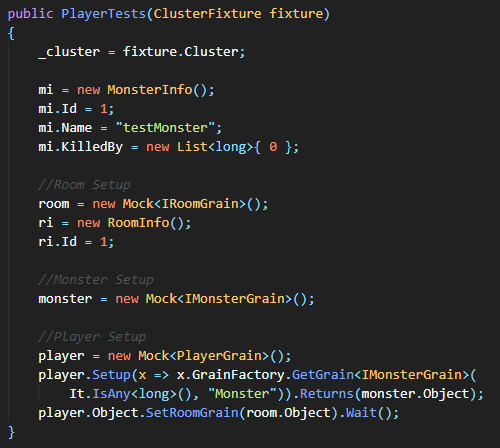
\includegraphics[width=0.7\linewidth]{Materials/TestingDiscussion/PlayerTestConstructor}
    \caption{The constructor for the player tests, showcasing how we chose to include the essentials for initialization.}
    \label{PlayerTestConstructor}
\end{figure}
If we look at \autoref{PlayerTestConstructor} we can see how we chose to setup the player tests. This setup is independent of the variation of the game we choose. Since we also have tests that are independent of variations, meaning they are included across all variations, the room mock and monster mock are initialized in the constructor. So, in tests that include the boss we chose to create the boss mock inside of those tests instead of in the setup alongside room and monster. There are two reasons for this. First off, as player does not include many boss tests we deemed it unnecessary to include in general setup. The second reason was to keep decomposition as simple as possible. If we keep the things affected by variations inside test cases we can decompose and combinate on a function level. This means, unlike in the grain decomposition, we do not have to insert lines of code here and there. This also means that the variations of abilities the player can take, fireball, roar and none, are not present in each others test. That is, for instance, fireball is not tested inside a damage test but these damage tests are kept separate. So, with this in mind, we can look at the CLS part of the tests and how we combinate those. \\
\\
Since tests of course are dependent on the grains, we can reuse some of the semantics from the grains. If we compare \autoref{semanticPlayerTest} to \autoref{SemanticTargetPlayer} from the subsection '\nameref{BuildPlayer}', we can see that they are similiar, however our semanticPlayerTestTargets differs in having another semantic type input in \textit{'playerTest}. 
\begin{figure}[h]
    \centering
    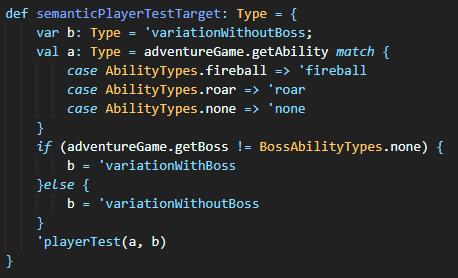
\includegraphics[width=0.7\linewidth]{Materials/TestingDiscussion/SemanticPlayerTestTarget}
    \caption{The function determining the semantic types for player tests.}
    \label{semanticPlayerTest}
\end{figure}
The reason we have the boss included in the semantic target is due to the fact that our player tests can be split in five parts. The first part of \autoref{semanticPlayerTest}, that is the pattern matching, would suffice for the first three parts of the player tests, which are the essential tests that will be included in all variations, the tests specific for roar and the tests specific for fireball. Then we have a test dealing damage to the boss. Most notably, one of our test cases include casting a fireball on the boss. That specific test is both dependent on a boss being present in the game variation and that the player ability is of type fireball. Only when those two criteria are fulfilled can we include that test. So with variations that vary both on the player's abilities and the presence of the boss, how did we combinate\todo{hedder det bare combine?} this? \\
\\
Before going into the semantics and structure of the player unit tests in our repository, we want to provide the reader with an overview of this structure, as it is somewhat complicated and a textual explanation may not suffice. We have provided a taxonomy of the player unit tests semantics, as can be seen in \autoref{taxonomyPlayerUnit}
\begin{figure}[H]
	\centering
	\begin{tikzpicture}[grow=down, -stealth]
	\node[bag]{Player Unit Test} 
	child[dashed]{;\node[bag]{testAbility}
		child[dashed]{; \node[bag]{bossPresent}
			child[dashdotted]{; \node[bag]{boss} % Dash eller solid?
				child[solid]{; \node[bag]{varWithBoss}}
			}
			child[solid]{; \node[bag]{varWithoutBoss}}	
		}
		child[solid]{; \node[bag]{fireball}}
		child[solid]{; \node[bag]{roar}}
		child[solid]{; \node[bag]{none}}
	};
	\end{tikzpicture}
	\caption{Taxonomy describing semantics of the player unit tests, showcasing the more complicated and nested structure.}
	\label{taxonomyPlayerUnit}
\end{figure}
It should be noted here that this is a simple representation of the structure and not a comprehensive one. For instance, both testAbility and bossPresent contain the two kindings, boss and ability. While this taxonomy looks similiar to \autoref{taxonomy}, with the same 'is a' and 'has a' connections, it differs slightly. Here we introduce a dash and dotted connection, which works as an optional 'has a'. This means that bossPresent either has a boss or is a varWithoutBoss, but not both at the same time. \\
\\ 
Semantically, we have split these combinators into three parts: \textit{'boss}, which contains the tests that are only dependent on the boss being a part of the game. That is, these tests do not use the player's abilities, but only the boss. The next semantic type is \textit{'bossPresent}. These combinators include tests that rely both on the player's ability and the boss. However, since we only have a single case where these overlap, it is only the \textit{'bossPresent('fireball, 'variationWithBoss)} that actually inserts a test, as there are no tests of roar and boss. The last semantic type is \textit{'testAbility} which contains the tests that are only specific for the player's ability. With these three parts, we can succesfully combinate all the possible variations of player tests that vary depending on ability and boss presence. Because of this, we can then describe player tests as: 
%\textit{string $\cap$ testAbility $\to$ MyResult $\cap$ playerTest}, where \textit{string $\cap$ boss $\to$ string $\cap$ bossPresent} and \textit{string $\cap$ bossPresent $\to$ string $\cap$ testAbility}
\begin{align*}
	&\textit{string $\cap$ testAbility} \to \textit{MyResult $\cap$ playerTest} \\
	\text{where\quad} &\textit{string $\cap$ bossPresent} \to \textit{string $\cap$ testAbility} \\
	\text{and\quad} &\textit{string $\cap$ boss} \to \textit{string $\cap$ bossPresent}
\end{align*}\todo{finno? ikke align?}
%\textit{string $\cap$ boss, string $\cap$ bossPresent, string $\cap$ testAbility $\to$ MyResult $\cap$ playerTest}\todo{forklar bedre? Er det korrekt? Nej, ikke helt så simpelt}. \\
This structure of the combinators is only due to the fireball boss test, which means that this intermediate step with the type of \textit{'bossPresent} is only truly meaningful when it comes to the fireball and boss variation. Because of this way we did the player tests, there are somewhat empty intermediate combinators for the abilities roar and none. That is, no tests are to be implemented that relies on the roar ability and the presence of the boss. We could argue that this opens up for the possibility of changing roar in a way that affects the boss, such that we needed tests that are dependent on these two. If this was the case, these new tests could easily be inserted into the intermediate combinator. However, we will not and do not expect roar to change in such a way to affect the boss directly, given the nature of the ability. This means that this structure of the player test combinators may seem somewhat redundant, due to the fact that the intermediate step, that is the intermediate combinators, is only needed for one specific case. So, if we were to look at the combinators of roar isolated, the intermediate step may seem irrelevant or puzzling.
\subsubsection{Room \& Boss Unit Tests}
Since neither room test nor boss tests have this overlap between multiple variables, it means that these tests are much simpler to implement. Let us start by looking at the boss tests. \\
\\
Boss tests are rather simple, as they only rely on the variation of the boss' abilities. Since boss does not take player or room into account, it makes for an easy synthesis. In essence, we only need one combinator for each of the boss' abilities for testing. Semantically, these combinators are of type \textit{'bossTest} that takes a kinding to specify which combinator to be chosen for synthesis. This means that boss tests can be described as: \textit{string $\cap$ bossTest $\to$ MyResult $\cap$ bossTestAbility}. However, this is not complete. \todo{Complete?} \\
The boss can have three different abilities: heal, DR (damage reduction) and none. The interesting ability here is none. None does not specify that the boss has no abilities, but instead it specifies that the boss is not present in this variation of the game. This means that the essential tests, that are independent of the boss' abilities, are no longer necessary and hence should not be included. This means in the case of no boss we do not need our \textit{'bossTest} to specify the tests that should be included based on abilities. This means we need a combinator that creates an empty file, such that no tests of the boss are present. This way, in the case where boss is nonexistent, boss tests can be described as: \textit{MyResult $\cap$ bossTestAbility}. \todo{Not sure how to show void $\to$ something. It would be intersected by 'none no?} \\
As the only factor of how the boss tests vary depends on the boss' abilities, tests of new abilities could easily be integrated as long as these tests are on a function level, such that this structure of \textit{'bossTest} can be kept. By doing this, scaling of the tests, based on new inclusion of abilities, seem feasible as the combinators do not intertwine and affect each other, a new combinator can simply be added for a given new ability. \todo{det er en kringle npnp. Lyder fint} %This also reinforces the idea that loose coupling makes for good combinators and thus this kind of unit testing is great in use of the CLS.
\\ \\
As the weather has been tested as its own class during unit testing, the room only need to take boss into account when being combinated. Other than the essential room tests, the only tests that vary from variation to variation is the boss part of room. This means that our semantic target for room only have two real cases, a \textit{'roomTestFile} with \textit{'boss} or with \textit{'noBoss}. Besides this, room is largely similiar to the boss tests in structure, where we have the semantic type \textit{'roomTest} that specifies a combinator with or without a boss. Therefore we can describe room tests as: \textit{string $\cap$ 'roomTest $\to$ MyResult $\cap$ 'roomTestFile}. 
\subsubsection{Integration Tests}
We have seen in \autoref{integrationDia} how we chose to implement integration testing with the bottom-up approach. The way we make integration tests is by testing one connection, for instance room and monster, then add player. This means that in PlayerIntegration tests we only test the remaining connections between the player, room and monster. This way, unlike unit tests, we no longer have to test the fireball / boss connection with player and boss in the PlayerIntegration, as this is now a connection to be tested when boss gets integrated, that is, during the BossIntegration. Because of this, player now only varies on the player abilities, as room and monster are default implementations that do not get altered \todo{hvad med weather tests? Godt spørgsmål :s}. So now PlayerIntegration is fairly simple to decompose and combinate, as we only have three non-overlapping cases to look at, that is the abilities: fireball, roar and none. The structure of PlayerIntegrationTests in our repository resembles the structure of the boss. Again, we have the semantic type \textit{'playerIntegrationAbility} of a given ability, that corresponds to the combinator that contains the tests specific for that ability. Since we kept the same structure as the unit tests, the essential tests that do not vary from variation to variation is already included in the file to be combinated, meaning that if we have \textit{'playerIntegrationAbility('none)} we get a combinator with an empty string, as no tests are to be added. We can describe PlayerIntegrationTests as: \textit{string $\cap$ 'playerIntegrationAbility $\to$ MyResult $\cap$ 'playerIntegration}. \\
%\\
%\begin{figure}[H]
%	\centering
%	\begin{tikzpicture}[grow=down, -stealth]
%	%\hspace{-2cm}
%	\node[bag]{Boss Integration Test} 
%	child[dashed]{;\node[bag]{bossIntegrationPlayerAbility}
%		child[solid]{; \node[bag]{None}}
%		child[solid]{; \node[bag]{Fireball}}
%	}
%	child[dashed]{;\node[bag]{bossIntegrationAbility}
%		child[solid]{; \node[bag]{DR}}
%		child[solid]{; \node[bag]{heal}}
%	};
%	\end{tikzpicture}
%	\caption{Taxonomy describing semantics of the boss integration tests, showcasing the simpler structure in comparison to the player unit tests.}
%	\label{taxonomyBossIntegration}
%\end{figure}
\begin{figure}[H]
	\centering
	\begin{tikzpicture}[grow=down, -stealth]
	\node[bag]{Boss Integration Test} 
	child[dashed]{;\node[bag]{bossIntAbility}
		child[dashed]{; \node[bag]{bossIntFireball}
			child[dashdotted]{; \node[bag]{ability} % Dash eller solid?
				child[solid]{; \node[bag]{fireball}}
			}
			child[solid]{; \node[bag]{none}}	
		}
		child[solid]{; \node[bag]{DR}}
		child[solid]{; \node[bag]{heal}}
		child[solid, thick]{; \node[bag]{none}}
	};
	\end{tikzpicture}
	\caption{Taxonomy describing semantics of the boss integration tests, showcasing how we have the same structure as our player unit tests.}
	\label{taxonomyBossIntegration}
\end{figure}
Now, since the connection of player and boss is tested during the BossIntegrationTests, this now resembles the same structure as the player unit tests. As with the playerTest, we have provided a diagram of bossIntegrationTests' taxonomy, which may help the reader more easily navigate the semantic structure as discussed. This can be seen in \autoref{taxonomyBossIntegration}. Here we have a new, thick line, which means that if bossIntAbility is a type none, we do not have a bossIntFireball connection. \\
In these boss integration tests, we need to take the player abilities into account, along with the boss abilities. Furthermore, because we may have a variation that does not contain the boss, we do not have boss unit tests and therefore we should neither have boss integration tests. This, just as in boss unit tests, also needs to be accounted for. 
As with the player unit tests, this structure requires the same intermediate step, because we have a test of the player fireball combined with the boss' damage reduction ability. If this was not the case, we would not require the intermediate step but rather have boss integration tests consisting of a player ability as well as a boss ability. In short, we have the same structure as player unit tests as we have the same overlap issue.
%However, we do not need the same intermediate step as in player unit tests, to account for the fireball boss test, as in this case, if we do not have a boss, we do not have boss integration tests at all and thus it is implied that if we do not combinate an empty boss integration file, we do indeed have a boss. 
%As such, tests that are dependent on specific player abilities can be combinated alongside the tests specific to boss abilities as these do not overlap as they did in player unit tests. 
\begin{figure}[]
    \centering
    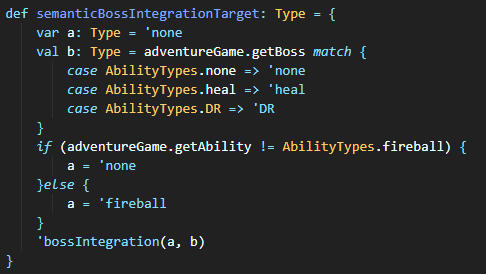
\includegraphics[width=0.6\linewidth]{Materials/TestingDiscussion/semanticBossIntegrationTarget}
    \caption{The function that specifies the boss' integration semantic targets, depending on boss abilities and player abilities.}
    \label{semanticBossIntegration}
\end{figure}
We can see in \autoref{semanticBossIntegration} the semantic target for boss integration tests. Here we can see, that like the player unit tests, we have an extra variable that depends on the player abilities. In this case, as we only have a connection between player and boss that depends on the player's fireball ability, we only have to check whether the variation includes this ability or not. However, it could easily be extended to a match case that includes the rest of the player abilities, if we made other abilities, or changed the current ones, such that other abilities than fireball had a connection with the boss and thus its integration tests. \\
Let us go over the semantics of boss integration tests. The tests specific to the player abilities, that is in our case either fireball or none, can be described as \textit{'bossIntegrationPlayerAbility}. The boss' abilities that include heal, DR and none are described as \textit{'bossIntegrationAbility}. The intermediate step, the tests depending on both player ability and boss ability are described as \textit{'bossIntegrationFireball}.
%With this in mind we can describe boss integration tests as: \textit{string $\cap$ 'bossIntegrationPlayerAbility, string $\cap$ 'bossIntegrationAbility $\to$ MyResult $\cap$ 'bossIntegration}. 
With this in mind, we can describe the boss integration tests the same way as player unit tests:
\begin{align*}
&\textit{string $\cap$ bossIntegrationAbility} \to \textit{MyResult $\cap$ bossIntegration} \\
\text{where\quad} &\textit{string $\cap$ bossIntegrationFireball} \to \textit{string $\cap$ bossIntegrationAbility} \\
\text{and\quad} &\textit{string $\cap$ bossIntegrationPlayerAbility} \to \textit{string $\cap$ bossIntegrationFireball}
\end{align*}
However, we also have the case with no boss integration tests at all, if we have any player ability, but the specific boss ability none. In this case, boss can simply be described as: \textit{MyResult $\cap$ 'bossIntegration}. \\
\\
In short, the way we chose to perform integration tests, the bottom-up approach, with the classes with least dependencies at the "bottom", proved to be the right choice as this made the integration tests easier for synthesis by implementing some connections later than others, that made for simpler combinators. However, we can see how the boss integration test has the same structure as the player unit tests, where both had to take each other into account due to the presence or abilities given, meaning that in this case, we only pushed this structure over to the boss integration tests instead of the player integration tests. \\
We can say that integration testing was a success synthesis-wise, atleast in our case with the adventure game, as all the integration tests made for fairly simple decomposing and combinators. This means that the tests are scalable, in the case of adding more variations to the game, atleast when it comes to the boss abilities and player abilities. However, just like with the unit tests, we still need to take care when it comes to overlaps, that is tests with multiple variation factors.
\subsubsection{Testing during Development}
So far, we have looked at how unit tests and integration testing has been implemented, decomposed and combinated with CLS, making tests that conform to specific variations of the adventure game. Let us take a step back and look at the tests more specifically for a moment. Now that we have made it clear how the tests have been incorporated into our repository, let us discuss more about the testing itself, what we have accomplished with it and how it has helped us doing development. \\
In \autoref{BuildRep} we discussed the implementation of grains in with CLS and how we came to the conclusion that accepting dead code would make it easier to decompose the grains. One may then ask, how do we ensure that this dead code is in fact unreachable or atleast how can we be sure that it does not create any obvious flaw in our variations where the dead code resides. More generally one could ask, how do our test overall ensure that our variations actually work as intended. \\ 
Let us examine the question, how can we somewhat reliably state that dead code does not crash our code? We can take the example of the dead code in \autoref{PlayerTakeDamage} that is, the if statement with roarActive inside player's TakeDamage function, in the variations where we do not have roar. We can see in \autoref{IntegrationTakeDamage} how we tested the player's takeDamage.
\begin{figure}[]
    \centering
    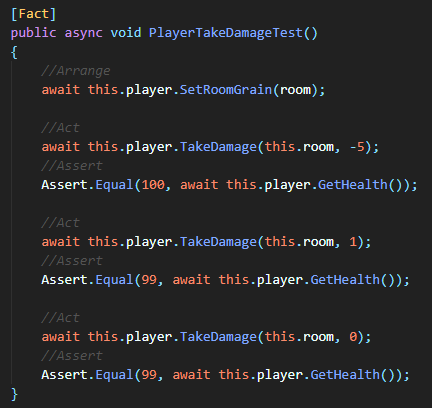
\includegraphics[width=0.6\linewidth]{Materials/TestingDiscussion/IntegrationTakeDamage}
    \caption{player's takeDamage in integration tests}
    \label{IntegrationTakeDamage}
\end{figure} 
As we only do black-box testing, we do not directly check the statements taken in TakeDamage while we test it. Instead, as we have mentioned in \autoref{TestTheory}, we use equivalence classes and boundary testing to examine how our TakeDamage reacts to different input. This way we cannot say that the dead code will never cause problems, but we have tested the function with input from our equivalence classes such that we can deem it unlikely that this code will affect the program with the input that we can expect the TakeDamage to receive doing runtime. \\ \\
Other than testing as an end product and as a result of synthesis, we can also look at how it helped us during development of our grains and their functionality. As we tested alongside development of our grains, the tests gave us valuable insight into problems or bugs that appeared as we implemented functionality, but also ways to simplify our code, which helped as a way to make grains simpler for decomposition \todo{hedder det decomposing?}. As a small example, originally the player was to implement a heal function, such that upon entering a sunny room, the player's heal function would be called. However, this was the only use for this function. As testing exposed the fact that we could take negative damage that would result in healing the player instead, we scrapped the heal function and used TakeDamage instead. \\
Even though we have used these black-box testing methods, our testing is not complete. As we will discuss in the next section, making tests with orleans and mockup did not go flawlessly and some of the functions proved difficult or downright impossible to test, atleast during unit testing. we will look at some of the obstacles that came during testing and what we did to work around or solve this in the next section. 
% Tests selv
%\subsubsection{Tests \& CLS}


\subsection{Obstacles}
Let us look at some of the obstacles we faced when creating tests. Some of these obstacles are specific to our grains, while other problems are more general. We will start by looking at the obstacles that are specific to the Orleans and Moq frameworks.
\subsubsection{GrainFactory} \label{GrainFactorySection}
In our grains we make use of GrainFactory to get the various grains in our adventure game for us. The way GrainFactory.GetGrain functions is that it looks through our silo, given a specified input id, and returns the grain, such that we can interact with it and call its functions. However, if we specify an id and our silo does not contain a grain corresponding to this id, it will not ignore or discard our request, but it will create a new grain for us and continue as planned. \todo{as explained in section 1.4 (?) about virtual actors} This is a problem when it comes to testing. As we mentioned and explained in the subsection '\nameref{MockingSection}', to perform unit testing on our grains, we mock the grains that it depends on and communicates with. 
\begin{figure}[h]
    \centering
    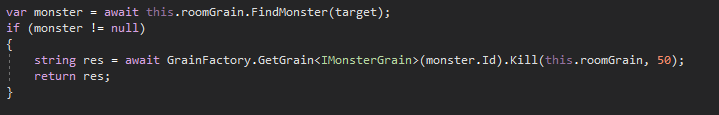
\includegraphics[width=\linewidth]{Materials/TestingTheory/FireballGrainFactory}
    \caption{Snippet of player's Fireball() function, showcasing the problem with GrainFactory. Even if our room was mocked and returned our mocked monster's id, GrainFactory would create a real monster based on this id, as it finds no monsters with this id.}
    \label{fireballGrainFactory}
\end{figure}
As we can see in \autoref{fireballGrainFactory}, our use of GrainFactory resides within some of the functions we wish to test in isolation. This means that if we wish to test this function in isolation from the other grains, we would create a mocked version of the monster, such that no real grain interferes in our test. However, the way GrainFactory works, this is not possible right out of the box. In our case, our GrainFactory would simply create a new monster grain for us, ignoring our mocked monster meant for the test and thus breaking our isolation of grains in the tests. So how do we get around this? We mock GrainFactory. \\
\\
As we went over in the subsection '\nameref{MockingVsSection}', mocking a class means our mock is an inherited class that uses the base implementations. To override a function in an inherited class, the function must be of type virtual or abstract. Since the original GrainFactory contains neither of those modifiers, we will have to override the function in our grains. This means that in each of our grains we implement a 'public new virtual IGrainFactory GrainFactory' that fetches the base GrainFactory. By doing this, we can mock the grains' GrainFactory properties such that when GrainFactory is called doing a test, we return a specified mock instead of a new grain and this have thus enabled us to sidestep GrainFactory and keep our tests isolated. The downside to this is, of course, that our way of sidestepping this obstacle is by writing code in the grains that have no other use than in testing. In other words, this way of overcoming the obstacle included making test specific code, which is a bad practice\todo{cite. Only know the slides stating it}. \\
However, GrainFactory is our way of communication between grains and thus used in a lot of the functions across the grains. Because of this, we deemed it a necessary implementation, as exclusion of this mock would greatly decrease our possible tests, by making a range of functions across the grains unavailable for testing due to inclusion of GrainFactory.
\subsubsection{GetPrimaryKey} \label{getPrimaryKey}
In the player's TakeDamage() function we make use of the room's GetPrimaryKey to ensure that we are in the same room where we took damage. If we are not in the same room, we have dodged the attack and should not take any damage. This is due to the distributed nature of our game. As we cannot predict in what order and time the messages arrive in, we have to take into account the possibility of an attack originating from a room we are no longer in. Thus if this is the case, we dodge the attack. The GetPrimaryKey fetches the ID of the specified grain. \\
This created some problems in testing however. GetPrimaryKey cannot be used by default in mocking of classes, meaning the comparison of GetPrimaryKey in TakeDamage() would fail and thus we could not test damage taken for the player. \\
Our initial idea here was to take the same route as with GrainFactory, that is mocking GetPrimaryKey, giving it some arbitrary value such that it would always pass the comparison and we could test damage taken in isolation. Apparently this is not possible, as GetPrimaryKey is non-overridable and inaccessible. This means that we would not be able to override it in the same way as GrainFactory and the mocking framework did not support use of GetPrimaryKey. Running tests that used GetPrimaryKey would give us an argument exception, stating that GetGrainIdentity was called by an unexpected type that was not a grain. We thought of other ways to do the comparison of room IDs, for instance with a public function that would return room's ID from RoomInfo. We ultimately decided against this, because this would be too much alteration of code for the sole purpose of testing, which again is bad practice and should be avoided. The reason we decided against this, and not with GrainFactory, is due to the fact that the GetPrimaryKey comparison is only used in the case of TakeDamage, hence it is not vital for a lot of the tests. \\
With no apparent way around this issue, it means that currently the tests that use the TestDamage function in unit tests will fail. Fortunately, this only makes two tests fail, TakeDamageTest() and RoarTest() in the player unit tests. Since we do not use mocking during integration testing, we do not face the issue of GetPrimaryKey in these cases, meaning that TakeDamage can be used in integration testing without this error. 
\subsubsection{Room Tests and Weather} \label{roomTestsWeather}
We have already been over the room and weather combination in the section '\nameref{adventureGame}'. As a reminder, the connection works as follows. A room will have a combinated pool of weather to choose from. When a player enters a room, the room will then apply one of these weathers from the pool at random.\todo{Finno eller redundant?} This way, a player will be affected by a random weather effect whenever entering a room, even if the player exits and enters the same rooms. Two of these weather effects affect the player directly, by either dealing damage to or healing the player upon entering the room. This proved difficult to control during testing. \\
\begin{figure}[h]
    \centering
    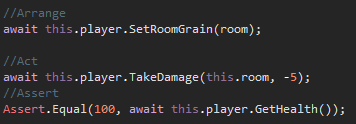
\includegraphics[width=0.5\linewidth]{Materials/TestingDiscussion/HailingWeatherDamageTest}
    \caption{An example of a player damage test that takes the weather into account. In this instance, because of the weather, we start with 95 health due to losing 5 by entering the room. What if the combinated game's seed chose the healing weather instead? Then the asserted health should be 115, and 105 if the weather did not affect the player.}
    \label{HailingWeatherDamageTest}
\end{figure}
During unit tests we use a mockup of the room interface, which means that the problem does not appear until the integration tests. What we did in the integration tests to keep the weather consistent was to use a predetermined seed in our random number generator, giving us the same weather in all the tests. This was not sufficient though, as this weather, that dealt 5 damage to the player, may or may not be in the pool in a given variation of the game. So, even with a predetermined seed, we will not be able to determine which weather is used for the testing. This means that all tests that uses or asserts the players health when taking damage may be skewed. For instance, as we initially tested with all weathers active, we always had the damage dealing weather, so all our tests take into account that we start off with 95 health versus the original 100 start health. We can see an example of a test taking the weather into account in \autoref{HailingWeatherDamageTest}. Let us say that we combinated a variation without this weather, such that no damage was dealt to the player. These tests would then fail. Essentially we have three types of weather, one that does not affect the player, one that deals damage and one that heals. How can we ensure we keep the weather consistent or separated from the tests that use room, without knowing what our pool of weather is going to be?  \\
Unfortunately, partially due to time restraints, we could not solve this issue or find a satisfactory workaround. As such, the tests that are influenced by the weather will not run successfully consistently. The tests, as they are now, depend on the weather being blizzard. As mentioned, the predetermined seed for the random generator is not sufficient when it comes to the variations, which may or may not include this rainy weather at all and thus we do not get one consistent weather (in our case, blizzard) in every variation when we run the tests.
\subsubsection{Newline Inconsistency}
It should also shortly be mentioned a minor problem we had, that we discarded as an unsolvable bug. Apparently, newline varies from operating system to operating system, meaning that a test could expect a "first line \textbackslash n second line", but the actual value is "first line \textbackslash r\textbackslash n second line". This means that some of the tests may fail even though they are virtually the same except for the inconsistency of newline. We deemed this problem or bug unimportant as it has nothing to do with Orleans or the CLS and thus it has been ignored.

%Funktioner vi ikke kunne teste?
\subsection{Summing Up} \label{summingUp}
%Goals?
%Test done their job?
%Test in CLS?
To sum up, we have looked at our tests in the perspective of the CLS, meaning how the different tests were decomposed and combinated. We have looked at how this was done both in unit tests and integration tests, while partially covering the effectiveness of these combinators and their structure. We also looked at the tests themselves, how they helped us during development and how they actually help reinforce our code's sturdiness, such that no apparent or obvious bug is present. However, as also covered, we looked at some of the obstacles when creating these tests, both from a synthesis perspective, but also just simply as the tests themselves and how some functions were made difficult to test. We looked over how we worked around some of these obstacles and how some of these were seemingly impossible to work around, at least without changing our code for the tests only. \\
Now that we have covered all these subjects, one may ask, have we been successful in testing and in synthesizing these tests with the CLS? This question has two parts. The first part is the testing itself and how efficiently our code has been tested. The second part is the CLS part, with how well our tests have been decomposed and synthesized, that is, how well does unit testing and integration testing work with the CLS, especially in our case and according to how we implemented them. \\
\\
Let us examine the first part. Have we succeeded in creating tests that efficiently test the correctness of our code? Have we managed to ensure that dead code does not make any apparent or obvious problems with our code? We have already touched upon these questions as we mentioned the benefits of our tests during our development. Here we mentioned how we tested for dead code by using the principles covered in the testing theory section, both in integration tests and the unit tests. So, by using boundary conditions and equivalence partitions, have we successfully tested for the influence of dead code to a satisfactory extent? Well, not entirely. As should be apparent from our section about obstacles in testing, we were not able to cover all the functions. Due to the high coupling between the grains, we had to use mockups for use in unit testing. However, some of the grains could not be fully mocked and as such, we ran into some problems that prevented us from testing certain functions. For instance, the player's TakeDamage function, which is a central part of the player, could not be tested in unit tests, as GetPrimaryKey could not be mocked and as such it gave us an error as the mock tried to access this. On the other hand, with integration tests, we did not rely on mockups and as such did not run into this problem, such that the player's TakeDamage function could successfully be tested in the integration part of the testing. In general, a big part of our troubles with testing stemmed from the use of mockups and how they could not entirely mock grains. However, this was of course not the only reason for our troubles as is apparent from our section on obstacles. \\
In short, as we have been unable to fully test the program, we have only somewhat accomplished testing the correctness of our code. In hindsight, if we had had focus on resolving the high coupling earlier in the process, we might have been able to test better in isolation, that is unit tests. On the other hand, our integration tests, without the mockups, proved easier to implement and we did not run into similar problems when creating these. So, while we would argue that a large part of the program, especially the parts made for variation, have successfully been tested for, some parts of the program was downright impossible to test without interfering with our code and as such, our testing is noncomprehensive and only somewhat satisfactory. \\
\\
Let us now examine the second part. Have we succeeded in synthesizing the tests and how well does our test scale when it comes to the CLS? We have already partially been over this, when we looked at the implementation of unit tests and integration tests in our repository. Because we kept the tests isolated in terms of requirements per test, meaning we only initialized essential parts in the setup, the tests were generally easy to decompose. For instance, as we mentioned, all tests that required the use of boss under player tests, were created specifically in those tests, such that when we decomposed tests, we could do this on a function based level, and thus keeping the ability tests easily separated. Most of the unit tests and integration tests were easily incorporated into our repository and we succesfully connected the tests to the grains, such that creating a specific variation of the game would correctly include the tests specific of that variation as well. As we also went over, most of the tests were also scalable, combinator-wise, in the way that adding new variations of abilities for the boss and player, and specifically tests thereof, could easily be added to the repository, without breaking the current structure of the combinators. \\
\\
The only issue we had with testing in accordance with CLS was the case of the player unit tests. We also mentioned this, how the overlap of the existence of the boss and the player's abilities, made the structure of the player tests combinators somewhat non-trivial and maybe not optimal. If we look at \autoref{testRoarBoss} we can see the case where our variation includes boss and the player ability roar.
\begin{figure}[]
    \centering
    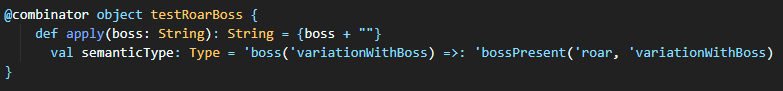
\includegraphics[width=\linewidth]{Materials/TestingDiscussion/testRoarBoss}
    \caption{The "intermediate step" of the player unit test combinator, when we have the variation where the player ability is roar.}
    \label{testRoarBoss}
\end{figure} 
In this specific combinator should be the tests that depend both on roar and boss. As there are no such tests, this combinator is empty. We discussed this earlier, where we came to the conclusion that there would never be a connection between roar and boss directly. This way, isolated, this case seems redundant as we could just have our normal roar tests here, but that would ruin the structure of the player tests. In short, due to one specific test, our entire structure of the combinators have to conform to this, which in all other cases, where the test is not to be included, may seem to be a redundant, but necessary, combinator. This seems somewhat non-scalable as new variations could include new dependencies and thus the entire structure could be changed. However, as stated, we only faced this issue in the player unit tests combinators, while the other combinators were more scalable. This is probably due to the dependencies that these combinators rely on and the nature of these dependencies.\\
\\
All in all, the unit tests and integration tests were remarkably easy to synthesize and as long as you watch out for overlaps that can complicate the synthesis process, this structure of tests makes for great combinators. In short, we would argue that we have succeeded in synthesizing the tests and they scale well as combinators as long as you keep dependencies in check.
% Section med sumup på tests i CLS? og Orleans? - Summing up our results and goals
%Implementation
%   - How we dealt with variations ?
%Obstacles
% - GrainFactory
% - GetPrimaryKey()
% - Weather     ?
% - Edgecases   ?
% - \r\n bug    ?
% - State testing omitted, måske keep it mello?
\section{Results}
We can now look into the results of our work and show how we can create our different variations of the game. As we have already discussed, we can give the player three different abilities and likewise we can give the boss two different abilities, but we can also choose not to have a boss. The room can take a combination of four weathers, and based on those, we can meet different weather effects in the game variations. We can thus create \textbf{36} different variations.

\begin{figure}[H]
	\centering
	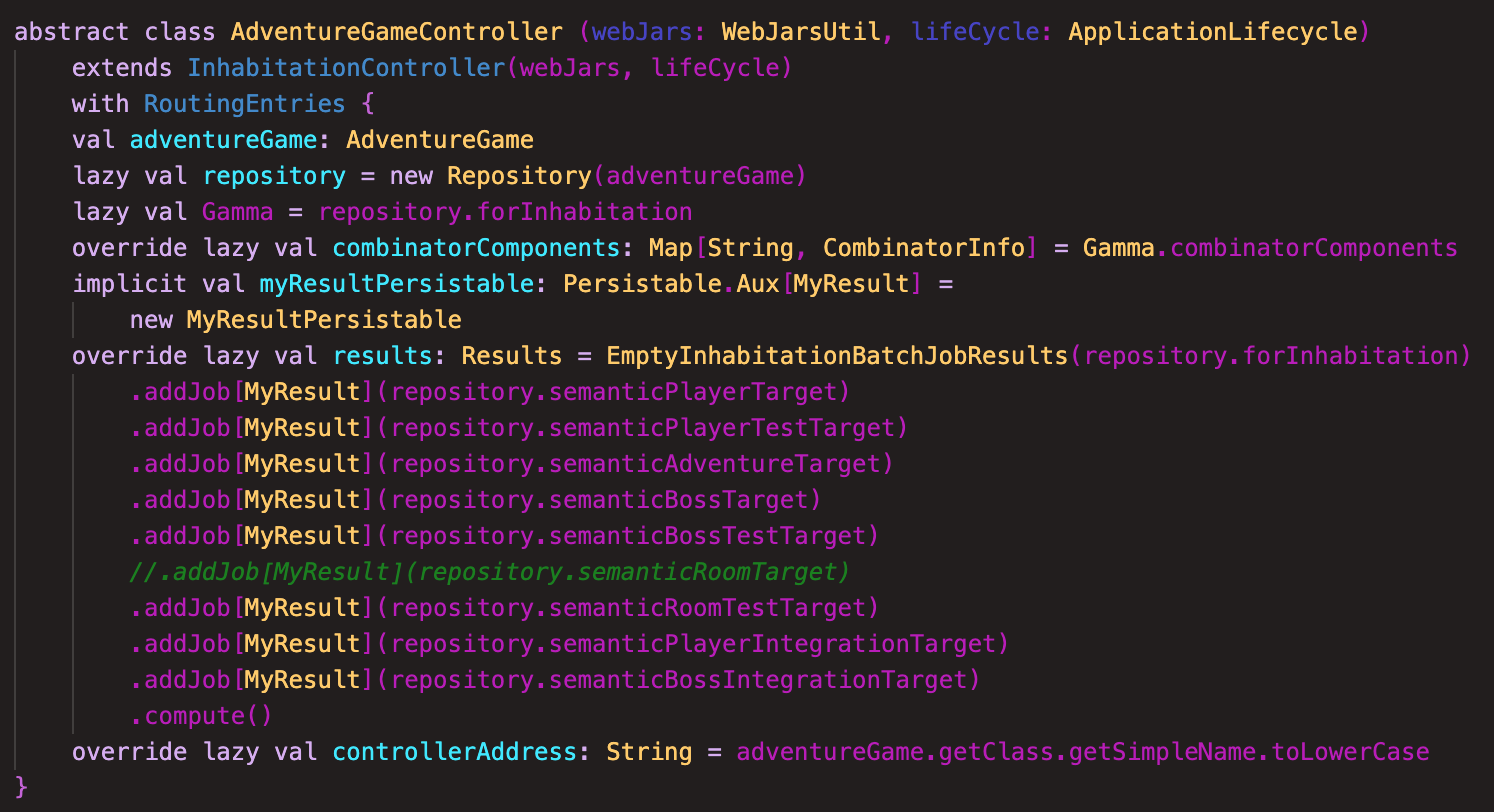
\includegraphics[width=\linewidth]{Materials/Results/AdventureController}
	\caption{In the \textit{AdventureGameController} we can see what jobs we are scheduling and thus what we want synthesized.}
	\label{Controller}
\end{figure}
In \autoref{Controller} we see \textit{AdventureGameController} in which we add the jobs we want done. Each job correspond to a synthesis we want done, and so if we are only interested in creating a player we could remove the other jobs.

\begin{figure}[H]
	\centering
	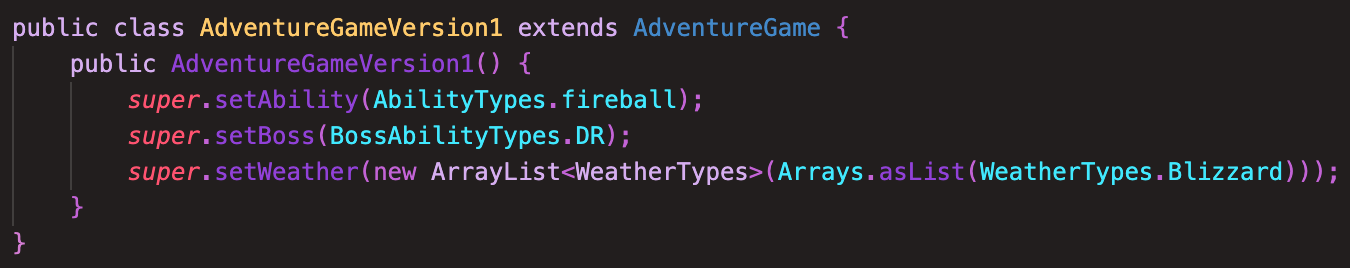
\includegraphics[width=\linewidth]{Materials/Results/AdventureVariation}
	\caption{By setting the \textit{AdventureGame} fields we can create different variation of our game. Here is shown a variation where the player has the fireball, the boss has the damage reduction ability and the possible weather effects would be blizzard.}
	\label{version1}
\end{figure}

To alter the variation we synthesize we need to look at a concrete class which extends our \textit{AdventureGame} class. We can here look at \textit{AdventureGameVersion1} which is seen in \autoref{version1}. We here see the player having the fireball ability, the boss having the damage reduction ability, and the possible weather effects being blizzard.

\begin{wrapfigure}{R}{0.6\linewidth}
	\centering
	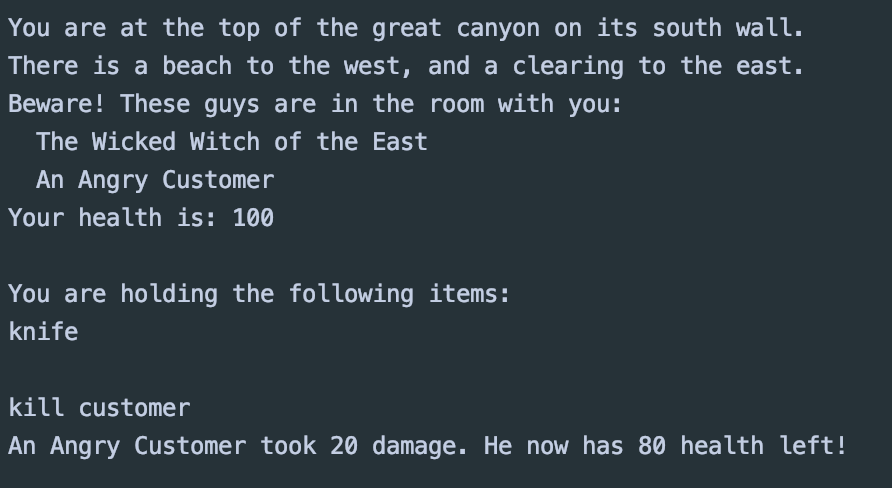
\includegraphics[width=\linewidth]{Materials/Results/AttackingCustomer}
	\caption{We see that the player with the knife can attack the Angry Customer.}
	\label{sc1}
\end{wrapfigure}
In the following we will showcase that the initial application can be synthesized and played. Here we are focusing on \autoref{sc1}, \autoref{sc2} and \autoref{sc3}. As we start the game we see that we cannot hit other players in the room with us. This is because we need the knife to attack with, as we do not have the fireball in the initial application. With the knife we can now begin stabbing both other players, but also the evil customer monster. The concept for hitting the 'Wicked Witch' is the same, but here we need the water. As this is all there is to the game in the initial application, our showcase of the initial application is done.

\begin{figure}[H]
	\centering
	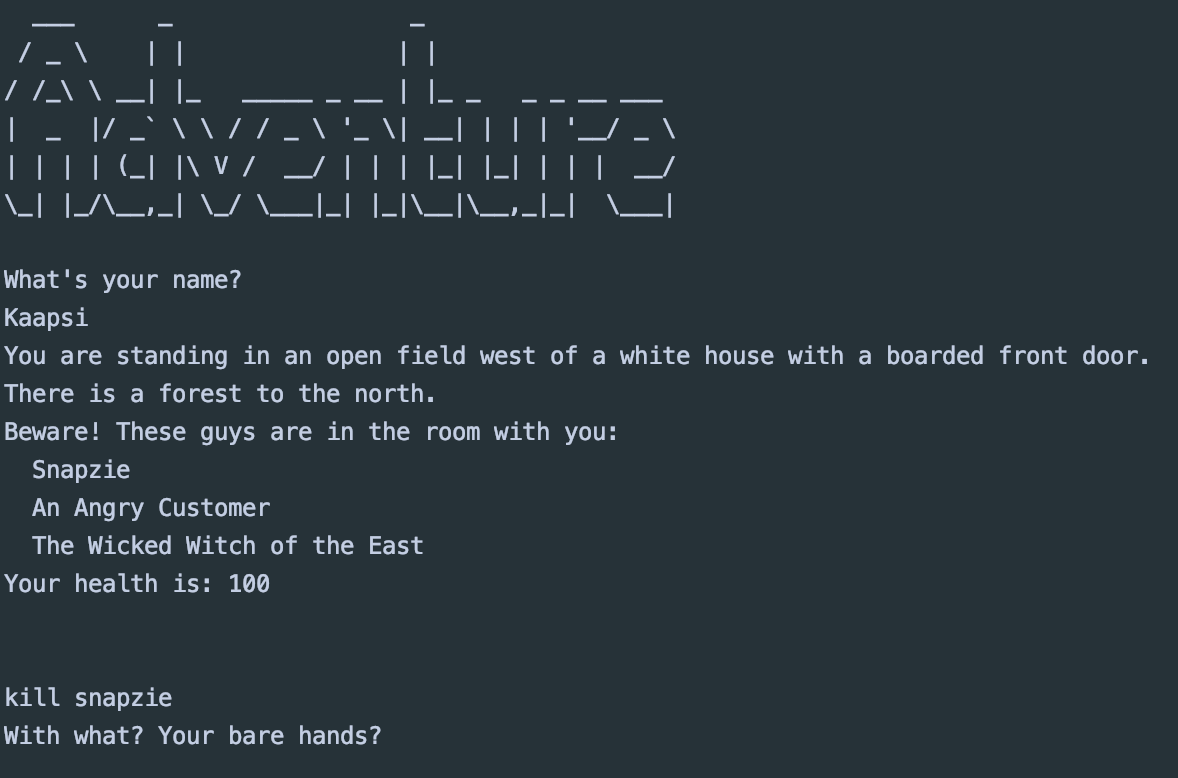
\includegraphics[width=0.9\linewidth]{Materials/Results/PlayersEntering}
	\caption{We see that we cannot attack other players without having the knife.}
	\label{sc2}
\end{figure}

\begin{figure}[H]
	\centering
	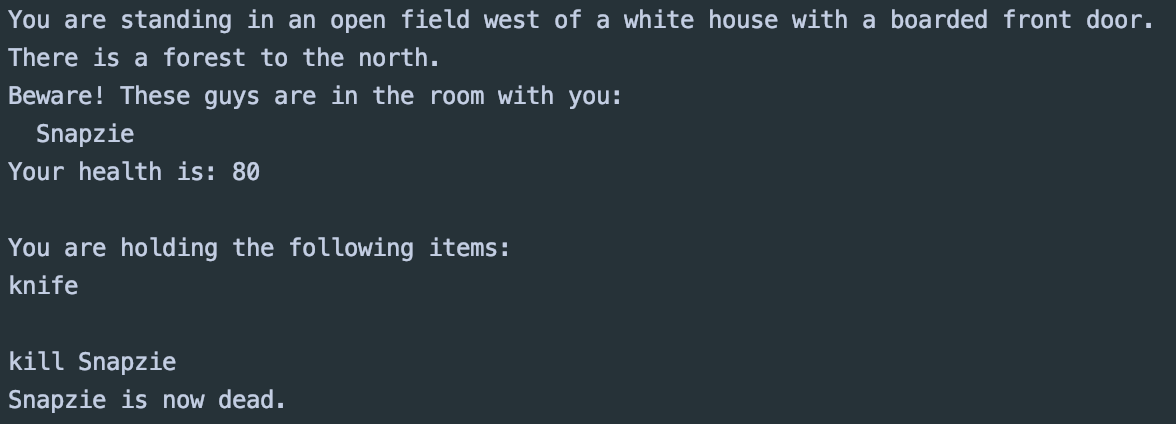
\includegraphics[width=0.8\linewidth]{Materials/Results/AttackingPlayer}
	\caption{We see that the player with the knife can attack other players.}
	\label{sc3}
\end{figure}

But to show off the weather effects and the boss, we have provided to more showcasing images for these variations, namely \autoref{sc4} and \autoref{sc5}.

\begin{figure}[H]
	\centering
	\includegraphics[width=0.6\linewidth]{example-image-c}
	\caption{We here see the effect of one the possible weathers.}
	\label{sc4}
\end{figure}

\begin{figure}[H]
	\centering
	\includegraphics[width=0.6\linewidth]{example-image-a}
	\caption{We here see the player fighting the boss.}
	\label{sc5}
\end{figure}

\begin{wrapfigure}{L}{0.4\linewidth}
	\centering
	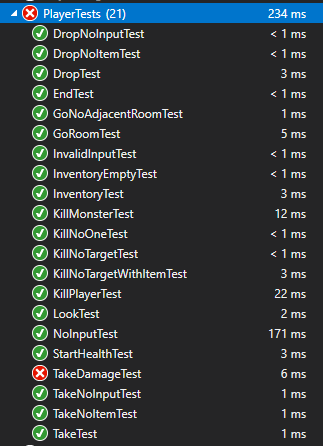
\includegraphics[width=\linewidth]{Materials/Results/PlayerUnitTestsInitial}
	\caption{A run of the tests, as they appear in the synthesized initial application.}
	\label{PlayerUnitInit}
\end{wrapfigure} 
Let us look at the results when it comes to testing. We have succeeded in creating the variations as explained above, including the corresponding tests. We add the tests as an individual job in the AdventureGameController. For instance, we can see in \autoref{Controller} how we both have a job for semanticPlayerTarget as well as semanticPlayerTestTarget. These are the player unit tests. \\
To test the initial application this way, we would need to synthesize it first. If we look at \autoref{version1}, we can set the different variables that create our variations of the game. In the case of the initial application, we would then have to set both setAbility and setBoss to their none types, as well as an empty setWeather.
In \autoref{PlayerUnitInit} we can see an example of one of the test suites run in the synthesized initial application, which is the player unit tests. These tests that appear in the initial application, without any variation will thus also appear in every variation of the game, meaning that variation only adds more tests. Earlier in the thesis, we have referred to these as the essential tests because of this.
As we can see, all these tests succeeded, except the TakeDamage test. We went over why this test does not succeed in the subsection \nameref{getPrimaryKey}. We can also compare this figure to our table \autoref{tableTests} and see how, unsurprisingly, the initial application of course contains fewer player unit tests than in the table. This is because the table contains the total number of tests, meaning all of them across the different variations. With this, we have successfully synthesized and run the tests for the initial application. Again, this does mean that some of the tests cannot run, but as with TakeDamage, this is not due to any fault in synthesizing of the grains or tests, but rather a fault in the tests themselves. That is, the TakeDamage test, for instance, did not run before synthesizing it either. \\
It should also be mentioned that while we do not have a boss in the initial application, bossTests and bossIntegrationTests are still created, but they are empty, they do not contain any code or tests. This is due to the nature of combinators, where we combinate empty boss files when a boss is not present. \\
Now that we have seen the synthesizing of the initial application was a success, we can check other variations of the game and see how the tests react to this. For instance, if we keep the same setup as the initial application, but we apply the fireball to the player, we can see how the tests change. If we look at the player unit tests again, we can see how this variation with fireball contains the same tests with new ones added. With this variation, all the fireball tests have been added except one. This is the FireballTestBoss, that was not combinated due to the boss not being present. If we compare the player fireball variation to our initial variation's player unit tests in \autoref{PlayerUnitInit}, we now have 25 tests instead of 21. 4 of our 5 fireball tests have thus been added, where the fifth as mentioned was the FireballTestBoss. Thus, we have been successful in synthesizing tests such that the correct tests are included in the different variations. %\\
%At last we should mention that while the synthesization was successful, we did not manage to make all the tests run, due to flaws in the our creation of them. However, while TakeDamageTest fails consistently, 

\section{Conclusion}
\subsection{Synthesizing actor code}
Our driving force has been to:
\begin{enumerate}
	\item Synthesizing objects with timers.
	\item Synthesizing objects which disposes timers.
	\item Synthesizing an object which spawns actors.
	\item Defining a list of arguments in our meta language which then effects our synthesis. 
\end{enumerate}
We began our discussion of how we had build our repository by looking at how the player got extended with abilities which used timers to create a cooldown for the abilities. As we have been successful in synthesizing the player, we meet our first goal. We then looked into how we could dispose the recurring ability timers from the monsters and boss. We here found that the safest way of doing so, was to leave the \textit{kill} methods unsynthesized to guarantee that the monsters' and boss' lifecycle would always end by disposing the timers at the end of their \textit{kill} method. We thus conclude that we meet our second goal and that critical code is best left unsynthesized. The boss always have the ability to spawn small monsters to help him fight. This is done by initializing a new actor, and so we meet goal number three. Looking at the room we see it is possible to define a combination of four weathers in our metalanguage and have these defined weathers added to the game variation. We have thus also succeeded in meeting our fourth goal.\\
When we started working with the CLS, we thought it would replace the need for dependency injection. However, as we conclude our work, we realize that to achieve clean repositories, we need close to no coupling between objects, and thus good design and encapsulation. Dependency injection helps with encapsulation and to limit coupling, and so, when working with the CLS it is important to understand that it does not replace any software engineering principles, on the contrary it is even more important to follow them as otherwise the decompositions gets messy.\\
Did we achieve good decomposition? We can look at our decomposition from two angles. First we can see our decomposition as decomposing the game into the actors. But we can also take a step further and look at how the actors can be decomposed. When looking form the second perspective our components are not really clean. They do not conform to interfaces, they are \textit{very} specific and they lack purpose and meaning as we can not see the whole picture. As we have focused on synthesizing the actors, we choose to conclude on the basis of the first perspective. This does not mean it was the best solution, as if we had focused on reusability and to create standards which the smaller components could conform to, we would probably have achieved better results. We choose to evaluate our work on the first perspective as that has been our perspective. What we see is not flawless decomposition where each component is completely isolated, but we achieved components which conforms to interfaces and to some extent can be reused and extended further upon. To this we conclude that it is more than possible to synthesize actor code and that it seems both Orleans and the CLS strive to work with encapsulated and isolated code which has no to little coupling with other entities.
\begin{thebibliography}{9}
\bibitem{ActorModelPaper}
Karmani, Rajesh K. Agha, Gul. Padua, David (ed.). 2011. 'Actors', part of 'Encyclopedia of Parallel Computing'. Springer Science+Business Media. Downloaded: November 26, 2019.

\bibitem{TestingCodeComplete}
McConnell, Steve. 2004. 'Code Complete'. Microsoft Press 2. ed. Chap. 22.

\bibitem{TestingAdaptiveCode}
Hall, Gary. 2014. 'Adaptive Code via C\#'. Microsoft Press 1. ed. Chap. 4.
\bibitem{OrleansPaper}
Bernstein, Philip A. Bykov, Sergey. Geller, Alan. et. al. 2014. 'Orleans: Distributed Virtual Actors for Programmability and Scalability'. Microsoft Research. Available at: \url{www.microsoft.com}. Downloaded: December 8, 2019.

%%%%%%%%%%%%%%%%%%%%%%%%%%%%%%%%%%%%%% SHOULD BE DELETED %%%%%%%%%%%%%%%%%%%%%%%%%%%%%%%%%%%%%%%%%%%%%%
\bibitem{book}
Marchewka, Jack T. 2015. 'Information Technology Project Management - Providing Measurable Organizational Value'. Wiley 5. ed.

\bibitem{rigsrevision}
Rigsrevisionen. 13. september 2019. 'Beretning om udvikling af det nye inddrivelsessystem og tilslutning af fordringshavere'. \url{www.rigsrevisionen.dk}. Hentet: 28. oktober 2019.

\bibitem{ugeopgave2}
Mogensen, Sten. 12. september 2019. 'Ugeopgave 2'. \url{absalon.ku.dk}. Hentet: 28. oktober 2019.

\bibitem{ugeopgave3}
Mogensen, Sten. 19. september 2019. 'Ugeopgave 3'. \url{absalon.ku.dk}. Hentet: 29. oktober 2019.

\bibitem{waterfallVsAgile}
Glowtouch.com. 'Waterfall vs. Agile: The Good, The Bad and The Misunderstood'. \url{https://www.glowtouch.com/waterfall-vs-agile-good-bad-misunderstood/}. Hentet: 29. oktober 2019.

\bibitem{scrumMaster}
Andersen, Tania. 4. januar 2018. 'Agile metoder er i dag den herskende måde at udvikle software på. Men Scrum og andre agile teknikker er ingen garanti for succes'. \url{www.version2.dk}. Hentet: 29. oktober 2019.
%%%%%%%%%%%%%%%%%%%%%%%%%%%%%%%%%%%%%% SHOULD BE DELETED %%%%%%%%%%%%%%%%%%%%%%%%%%%%%%%%%%%%%%%%%%%%%%
\end{thebibliography}

\end{document}